% Options for packages loaded elsewhere
\PassOptionsToPackage{unicode}{hyperref}
\PassOptionsToPackage{hyphens}{url}
%
\documentclass[
  ignorenonframetext,
]{beamer}
\usepackage{pgfpages}
\setbeamertemplate{caption}[numbered]
\setbeamertemplate{caption label separator}{: }
\setbeamercolor{caption name}{fg=normal text.fg}
\beamertemplatenavigationsymbolsempty
% Prevent slide breaks in the middle of a paragraph
\widowpenalties 1 10000
\raggedbottom
\setbeamertemplate{part page}{
  \centering
  \begin{beamercolorbox}[sep=16pt,center]{part title}
    \usebeamerfont{part title}\insertpart\par
  \end{beamercolorbox}
}
\setbeamertemplate{section page}{
  \centering
  \begin{beamercolorbox}[sep=12pt,center]{part title}
    \usebeamerfont{section title}\insertsection\par
  \end{beamercolorbox}
}
\setbeamertemplate{subsection page}{
  \centering
  \begin{beamercolorbox}[sep=8pt,center]{part title}
    \usebeamerfont{subsection title}\insertsubsection\par
  \end{beamercolorbox}
}
\AtBeginPart{
  \frame{\partpage}
}
\AtBeginSection{
  \ifbibliography
  \else
    \frame{\sectionpage}
  \fi
}
\AtBeginSubsection{
  \frame{\subsectionpage}
}

\usepackage{amsmath,amssymb}
\usepackage{lmodern}
\usepackage{iftex}
\ifPDFTeX
  \usepackage[T1]{fontenc}
  \usepackage[utf8]{inputenc}
  \usepackage{textcomp} % provide euro and other symbols
\else % if luatex or xetex
  \usepackage{unicode-math}
  \defaultfontfeatures{Scale=MatchLowercase}
  \defaultfontfeatures[\rmfamily]{Ligatures=TeX,Scale=1}
\fi
\usetheme[]{simple}
% Use upquote if available, for straight quotes in verbatim environments
\IfFileExists{upquote.sty}{\usepackage{upquote}}{}
\IfFileExists{microtype.sty}{% use microtype if available
  \usepackage[]{microtype}
  \UseMicrotypeSet[protrusion]{basicmath} % disable protrusion for tt fonts
}{}
\makeatletter
\@ifundefined{KOMAClassName}{% if non-KOMA class
  \IfFileExists{parskip.sty}{%
    \usepackage{parskip}
  }{% else
    \setlength{\parindent}{0pt}
    \setlength{\parskip}{6pt plus 2pt minus 1pt}}
}{% if KOMA class
  \KOMAoptions{parskip=half}}
\makeatother
\usepackage{xcolor}
\newif\ifbibliography
\setlength{\emergencystretch}{3em} % prevent overfull lines
\setcounter{secnumdepth}{-\maxdimen} % remove section numbering


\providecommand{\tightlist}{%
  \setlength{\itemsep}{0pt}\setlength{\parskip}{0pt}}\usepackage{longtable,booktabs,array}
\usepackage{calc} % for calculating minipage widths
\usepackage{caption}
% Make caption package work with longtable
\makeatletter
\def\fnum@table{\tablename~\thetable}
\makeatother
\usepackage{graphicx}
\makeatletter
\def\maxwidth{\ifdim\Gin@nat@width>\linewidth\linewidth\else\Gin@nat@width\fi}
\def\maxheight{\ifdim\Gin@nat@height>\textheight\textheight\else\Gin@nat@height\fi}
\makeatother
% Scale images if necessary, so that they will not overflow the page
% margins by default, and it is still possible to overwrite the defaults
% using explicit options in \includegraphics[width, height, ...]{}
\setkeys{Gin}{width=\maxwidth,height=\maxheight,keepaspectratio}
% Set default figure placement to htbp
\makeatletter
\def\fps@figure{htbp}
\makeatother

\makeatletter
\makeatother
\makeatletter
\makeatother
\makeatletter
\@ifpackageloaded{caption}{}{\usepackage{caption}}
\AtBeginDocument{%
\ifdefined\contentsname
  \renewcommand*\contentsname{Table of contents}
\else
  \newcommand\contentsname{Table of contents}
\fi
\ifdefined\listfigurename
  \renewcommand*\listfigurename{List of Figures}
\else
  \newcommand\listfigurename{List of Figures}
\fi
\ifdefined\listtablename
  \renewcommand*\listtablename{List of Tables}
\else
  \newcommand\listtablename{List of Tables}
\fi
\ifdefined\figurename
  \renewcommand*\figurename{Figure}
\else
  \newcommand\figurename{Figure}
\fi
\ifdefined\tablename
  \renewcommand*\tablename{Table}
\else
  \newcommand\tablename{Table}
\fi
}
\@ifpackageloaded{float}{}{\usepackage{float}}
\floatstyle{ruled}
\@ifundefined{c@chapter}{\newfloat{codelisting}{h}{lop}}{\newfloat{codelisting}{h}{lop}[chapter]}
\floatname{codelisting}{Listing}
\newcommand*\listoflistings{\listof{codelisting}{List of Listings}}
\makeatother
\makeatletter
\@ifpackageloaded{caption}{}{\usepackage{caption}}
\@ifpackageloaded{subcaption}{}{\usepackage{subcaption}}
\makeatother
\makeatletter
\@ifpackageloaded{tcolorbox}{}{\usepackage[many]{tcolorbox}}
\makeatother
\makeatletter
\@ifundefined{shadecolor}{\definecolor{shadecolor}{rgb}{.97, .97, .97}}
\makeatother
\makeatletter
\@ifpackageloaded{sidenotes}{}{\usepackage{sidenotes}}
\@ifpackageloaded{marginnote}{}{\usepackage{marginnote}}
\makeatother
\makeatletter
\makeatother
\ifLuaTeX
  \usepackage{selnolig}  % disable illegal ligatures
\fi
\IfFileExists{bookmark.sty}{\usepackage{bookmark}}{\usepackage{hyperref}}
\IfFileExists{xurl.sty}{\usepackage{xurl}}{} % add URL line breaks if available
\urlstyle{same} % disable monospaced font for URLs
\hypersetup{
  pdftitle={Coasting on Duality},
  pdfauthor={Omar Lizardo},
  hidelinks,
  pdfcreator={LaTeX via pandoc}}

\title{Coasting on Duality}
\subtitle{What We Get When We Do Two-Mode Network CA}
\author{Omar Lizardo}
\date{5/22/24}
\institute{\emph{University of California, Los Angeles}}

\begin{document}
\frame{\titlepage}
\ifdefined\Shaded\renewenvironment{Shaded}{\begin{tcolorbox}[enhanced, frame hidden, sharp corners, borderline west={3pt}{0pt}{shadecolor}, boxrule=0pt, breakable, interior hidden]}{\end{tcolorbox}}\fi

\begin{frame}{CA and Two Mode Networks}
\protect\hypertarget{ca-and-two-mode-networks}{}
\begin{itemize}
\tightlist
\item
  While still not very common, Correspondence Analysis (CA) has been
  sporadically used in \emph{analyzing} two-mode network data*
\item
  But criticized for being limited and inapplicable for most ``SNA''
  tasks**

  \begin{itemize}
  \tightlist
  \item
    Computing (Centrality-Like) Measures of Node Position
  \item
    Computing Measures of Group Membership
  \end{itemize}
\end{itemize}

\marginnote{\begin{footnotesize}

*Breiger 2000; Roberts 2000; Faust 2005; D'Esposito et al.~2014

**Bonacich 1991; Borgatti \& Everett 1997

\end{footnotesize}}
\end{frame}

\begin{frame}{CA and Two Mode Networks}
\protect\hypertarget{ca-and-two-mode-networks-1}{}
\begin{itemize}
\tightlist
\item
  While still not very common, Correspondence Analysis (CA) has been
  sporadically used in \emph{analyzing} two-mode network data*
\item
  But criticized for being limited and inapplicable for most ``SNA''
  tasks**

  \begin{itemize}
  \tightlist
  \item
    Computing (Centrality-Like) Measures of Node Position
  \item
    Computing Measures of Group Membership
  \end{itemize}
\item
  CA Proponents point to some important advantages of CA for the
  analysis of two-mode networks:

  \begin{itemize}
  \tightlist
  \item
    CA can provide a ``joint display'' of the structural connectivity
    patterns in two-mode data
  \item
    (M)CA can be used to ``visually explore'' two-mode networks
  \end{itemize}
\end{itemize}

\marginnote{\begin{footnotesize}

*Breiger 2000; Roberts 2000; Faust 2005; D'Esposito et al.~2014

**Bonacich 1991; Borgatti \& Everett 1997

\end{footnotesize}}
\end{frame}

\begin{frame}{CA and Two Mode Networks}
\protect\hypertarget{ca-and-two-mode-networks-2}{}
\begin{itemize}
\tightlist
\item
  While still not very common, Correspondence Analysis (CA) has been
  sporadically used in \emph{analyzing} two-mode network data*
\item
  But criticized for being limited and inapplicable for most ``SNA''
  tasks**

  \begin{itemize}
  \tightlist
  \item
    Computing (Centrality-Like) Measures of Node Position
  \item
    Computing Measures of Group Membership
  \end{itemize}
\item
  This presentation builds on and expands on previous research on using
  CA for two-mode data analysis but discusses aspects of CA that have
  not been emphasized in previous research:

  \begin{itemize}
  \tightlist
  \item
    CA as computing a type of ``(Reflective) Dual Centrality'' on the
    entities in the two-modes*
  \end{itemize}
\end{itemize}

\marginnote{\begin{footnotesize}

*Rediscovered recently under the heading of the Economic Complexity
Index (ECI; Hidalgo and Hausman 2009)

\end{footnotesize}}
\end{frame}

\begin{frame}{CA and Two Mode Networks}
\protect\hypertarget{ca-and-two-mode-networks-3}{}
\begin{itemize}
\tightlist
\item
  While still not very common, Correspondence Analysis (CA) has been
  sporadically used in \emph{analyzing} two-mode network data*
\item
  But criticized for being limited and inapplicable for most ``SNA''
  tasks**

  \begin{itemize}
  \tightlist
  \item
    Computing (Centrality-Like) Measures of Node Position
  \item
    Computing Measures of Group Membership
  \end{itemize}
\item
  This presentation builds on and expands on previous research on using
  CA for two-mode data analysis but discusses aspects of CA that have
  not been emphasized in previous research:

  \begin{itemize}
  \tightlist
  \item
    CA as extracting ``positional'' information the entities in the two
    modes

    \begin{itemize}
    \tightlist
    \item
      With positions defined by ``Generalized Relational Similarity''
    \item
      Similarly central entities have similar patterns of connectivity
      with entities that are themselves similar**
    \end{itemize}
  \end{itemize}
\end{itemize}

\marginnote{\begin{footnotesize}

**Jeh \& Widom 2002; Kovacs 2010; Lizardo 2024

\end{footnotesize}}
\end{frame}

\begin{frame}{Southern Women Data}
\protect\hypertarget{southern-women-data}{}
table output

","

"{]},col:{[}2,"

","

"{]},tr:{[}2,"

","

"{]},td:{[}3,"

","

E1

E2

E3

E4

E5

E6

E7

E8

E9

E10

E11

E12

E13

E14

BRENDA

1

0

1

1

1

1

1

1

0

0

0

0

0

0

CHARLOTTE

0

0

1

1

1

0

1

0

0

0

0

0

0

0

DOROTHY

0

0

0

0

0

0

0

1

1

0

0

0

0

0

ELEANOR

0

0

0

1

1

1

1

1

0

0

0

0

0

0

EVELYN

1

1

1

1

1

1

0

1

1

0

0

0

0

0

FLORA

0

0

0

0

0

0

0

0

1

0

1

0

0

0

FRANCES

0

0

1

1

1

1

0

1

0

0

0

0

0

0

HELEN

0

0

0

0

0

0

1

1

0

1

1

1

0

0

KATHERINE

0

0

0

0

0

0

0

1

1

1

0

1

1

1

LAURA

1

1

1

0

1

1

1

1

0

0

0

0

0

0

MYRNA

0

0

0

0

0

0

0

1

1

1

0

1

0

0

NORA

0

0

0

0

0

0

1

0

1

1

1

1

1

1

OLIVIA

0

0

0

0

0

0

0

0

1

0

1

0

0

0

PEARL

0

0

0

0

0

1

0

1

1

0

0

0

0

0

RUTH

0

0

0

1

1

0

1

1

1

0

0

0

0

0

SYLVIA

0

0

0

0

0

0

1

1

1

1

0

1

1

1

THERESA

0

1

1

1

1

1

1

1

1

0

0

0

0

0

VERNE

0

0

0

0

0

0

1

1

1

0

0

1

0

0
\end{frame}

\begin{frame}{What do we get when we do CA?}
\protect\hypertarget{what-do-we-get-when-we-do-ca}{}
\begin{columns}[T]
\begin{column}{0.5\textwidth}
\begin{itemize}
\tightlist
\item
  Taken singly, the first dimension of CA suggests an \textbf{ordering}

  \begin{itemize}
  \tightlist
  \item
    Is this connected to centrality?
  \item
    If so, what is the relation (if any) to existing two-mode
    centralities?*
  \end{itemize}
\item
  Take jointly, the first two dimensions of CA suggest a
  \textbf{grouping}

  \begin{itemize}
  \tightlist
  \item
    Connected to group cohesion?**
  \item
    Affinity of actors for particular events?***
  \end{itemize}
\end{itemize}
\end{column}

\marginnote{\begin{footnotesize}

*Bonacich 1991

**Doreian 1979

***Faust 2005

\end{footnotesize}}

\begin{column}{0.5\textwidth}
\begin{figure}

{\centering 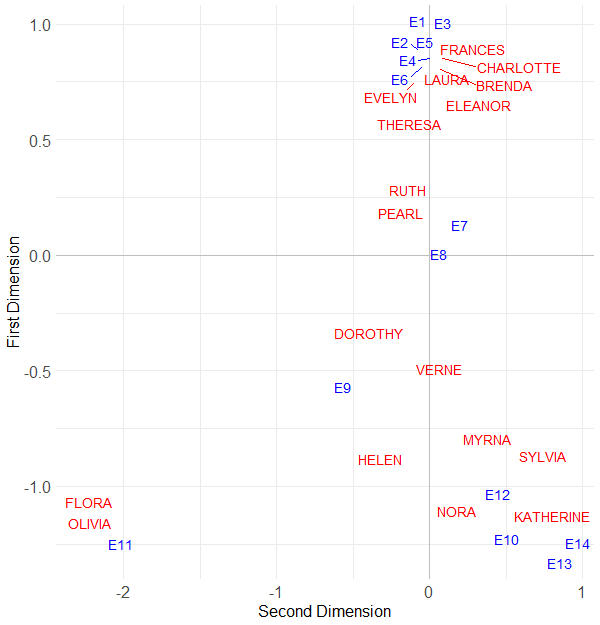
\includegraphics{Plots/ca-sw.png}

}

\caption{Correspondence Plot of Southern Women Data Obtained from Simple
CA of the Affiliation Matrix}

\end{figure}
\end{column}
\end{columns}
\end{frame}

\begin{frame}{What do we get when we do CA?}
\protect\hypertarget{what-do-we-get-when-we-do-ca-1}{}
\begin{itemize}
\tightlist
\item
  To (try to) shed light on these questions I examine the cases of three
  relatively recent ``accidental reinventions'' of CA in the ``network
  science'' and ``data science'' (computer and information science)
  literatures:

  \begin{itemize}
  \tightlist
  \item
    The ``Economic Complexity Index'' (ECI)*

    \begin{itemize}
    \tightlist
    \item
      Relevant to the question of centrality
    \end{itemize}
  \item
    \emph{SimRank} and Generalized Relational Similarity**

    \begin{itemize}
    \tightlist
    \item
      Relevant to the question of grouping
    \end{itemize}
  \end{itemize}
\item
  The ECI case has been examined in detail in recent work***
\item
  The second and third are new to this presentation

  \begin{itemize}
  \tightlist
  \item
    All shed light on what exactly we get when we use CA to analyze two
    mode data
  \end{itemize}
\end{itemize}

\marginnote{\begin{footnotesize}

*Hidalgo \& Hausmann 2009

**Jeh \& Widom 2002; Kovacs (2010)

***van Dam et al.~2021; Mealy 2019

\end{footnotesize}}
\end{frame}

\begin{frame}{CA and Reflective Centrality}
\protect\hypertarget{ca-and-reflective-centrality}{}
\begin{itemize}
\tightlist
\item
  Hidalgo \& Hausmann (2009) introduced a ``novel'' way to rank nodes in
  two-mode networks

  \begin{itemize}
  \tightlist
  \item
    Their approach, called ``reflective,'' was originally applied to
    country-by-product networks*
  \end{itemize}
\end{itemize}

\pause

\begin{itemize}
\tightlist
\item
  The method has since been shown to be applicable to other two-mode
  networks (like cultural networks)**
\item
  I introduce here using the more familiar sociological example of the
  \textbf{duality of persons and groups}***
\end{itemize}

\marginnote{\begin{footnotesize}

*Referred to as the Economic Complexity Index (ECI)

**Lizardo 2018

***Breiger 1974

\end{footnotesize}}
\end{frame}

\begin{frame}{CA and Reflective Centrality}
\protect\hypertarget{ca-and-reflective-centrality-1}{}
\begin{itemize}
\tightlist
\item
  Notation:

  \begin{itemize}
  \tightlist
  \item
    A two-mode network composed of a set of persons \(P\)
  \item
    Their affiliation relations to a set of groups \(G\)
  \item
    Represented by an affiliation matrix \(\mathbf{A}\)
  \end{itemize}
\end{itemize}

\pause

\begin{itemize}
\tightlist
\item
  \(\mathbf{A}\) is of dimensions \(|P| \times |G|\) with people along
  the rows and groups across the columns

  \begin{itemize}
  \tightlist
  \item
    \(|P|\) is the cardinality of the persons set\\
  \item
    \(|G|\) is the cardinality of the group set
  \end{itemize}
\end{itemize}

\pause

\begin{itemize}
\tightlist
\item
  \(\mathbf{A}\) has cell entries \(a_{pg}= 1\) if person \textit{p} is
  affiliated with group \textit{g} and \(a_{pg}= 0\) otherwise.
\end{itemize}
\end{frame}

\begin{frame}{CA and Reflective Centrality}
\protect\hypertarget{ca-and-reflective-centrality-2}{}
\begin{itemize}
\item
  If we are going to compute the centrality of nodes in a two-mode
  network, the most natural place to start is with the good old
  \textbf{degree centrality}*
\item
  Given this, the degree-centrality of people is given by:
\end{itemize}

\begin{equation}\protect\hypertarget{eq-dp}{}{
C^R_p(1) = \sum_g a_{pg}
}\label{eq-dp}\end{equation}

\begin{itemize}
\tightlist
\item
  And for groups:
\end{itemize}

\begin{equation}\protect\hypertarget{eq-dg}{}{
   C^R_g(1) = \sum_p a_{pg}
}\label{eq-dg}\end{equation}

\marginnote{\begin{footnotesize}

*Faust 1997, eqs. 4 and 5

\end{footnotesize}}
\end{frame}

\begin{frame}{CA and Reflective Centrality}
\protect\hypertarget{ca-and-reflective-centrality-3}{}
\begin{itemize}
\item
  Once we have the first-order quantities \(C^R_p(1)\) and \(C^R_g(1)\),
  we can compute ``second-order centralities'' \(C^R(2)\) for both
  people and groups
\item
  For people, these are given by:*
\end{itemize}

\begin{equation}\protect\hypertarget{eq-r2p}{}{
C^R_p(2) = \frac{1}{C^R_p(1)}\sum_g a_{pg}C^R_g(1)
}\label{eq-r2p}\end{equation}

\begin{itemize}
\tightlist
\item
  And for groups:**
\end{itemize}

\begin{equation}\protect\hypertarget{eq-r2g}{}{   
C^R_g(2) = \frac{1}{C^R_g(1)}\sum_p a_{pg}C^R_p(1)
}\label{eq-r2g}\end{equation}

\marginnote{\begin{footnotesize}

*People are central when the average sum of the size of the groups they
belong to is large

**Groups are central when the average activity of the people who belong
to them is large

\end{footnotesize}}

\note{Equation Equation~\ref{eq-r2p} says ``people are more central when
the average sum of the size of the groups they belong to is large'\,'
(e.g., whenever \(a_{pg} = 1\) and \(C^R_g(1)\) is a big number).
Equation Equation~\ref{eq-r2g} says''groups are more central when the
average activity of their members is large'' (e.g., whenever
\(a_{pg} = 1\) and \(C^R_p(1)\) is a big number).}
\end{frame}

\begin{frame}{CA and Reflective Centrality}
\protect\hypertarget{ca-and-reflective-centrality-4}{}
\begin{itemize}
\item
  Of course, once we have the second-order quantities \(C^R_p(2)\) and
  \(C^R_g(2)\), we can compute ``third-order centralities'' \(C^R(3)\)
  for both people and groups
\item
  For people, these are given by:
\end{itemize}

\begin{equation}\protect\hypertarget{eq-r3p}{}{
   C^R_p(3) = \frac{1}{C^R_p(1)}\sum_g a_{pg}C^R_g(2)
}\label{eq-r3p}\end{equation}

\begin{itemize}
\tightlist
\item
  And for groups:
\end{itemize}

\begin{equation}\protect\hypertarget{eq-r3g}{}{   
   C^R_g(3) = \frac{1}{C^R_g(1)}\sum_p a_{pg}C^R_p(2)
}\label{eq-r3g}\end{equation}

\marginnote{\begin{footnotesize}

*People are central when the average sum of the average activity of the
members of the groups they belong to is large

**Groups are central when the average sum of the average size of the
groups their members belong to is large

\end{footnotesize}}

\note{Equation Equation~\ref{eq-r3p} says something like ``people are
more central when the average sum of the average activity of the members
of the groups they belong to is large'' (e.g., \(a_{pg} = 1\) and
\(C^R_g(2)\) is a big number). Equation Equation~\ref{eq-r3g} says,
``groups are more central when the average sum of the average size of
the groups their members belong to is large.'' (e.g., \(a_{pg} = 1\) and
\(C^R_p(2)\) is a big number).}
\end{frame}

\begin{frame}{CA and Reflective Centrality}
\protect\hypertarget{ca-and-reflective-centrality-5}{}
\begin{itemize}
\item
  More generally, Hidalgo \& Hausmann show that we can define a
  \textbf{series} of reflective quantities*
  \(C^R_p(4), C^R_p(5)...C^R_p(q)\) and
  \(C^R_g(4), C^R_g(5)...C^R_g(q)\)
\item
  For people, these are given by:
\end{itemize}

\begin{equation}\protect\hypertarget{eq-rip}{}{   
C^R_p(q) = \frac{1}{C^R_p(1)}\sum_g a_{pg}C^R_g(q-1) 
}\label{eq-rip}\end{equation}

\begin{itemize}
\tightlist
\item
  And for groups:
\end{itemize}

\begin{equation}\protect\hypertarget{eq-rig}{}{   
C^R_g(q) = \frac{1}{C^R_g(1)}\sum_p a_{pg}C^R_p(q-1)
}\label{eq-rig}\end{equation}

\marginnote{\begin{footnotesize}

*Whose verbal and substantive interpretation becomes more elusive as the
number of iterations increases

\end{footnotesize}}
\end{frame}

\begin{frame}{CA and Reflective Centrality}
\protect\hypertarget{ca-and-reflective-centrality-6}{}
\begin{itemize}
\tightlist
\item
  For people:

  \begin{itemize}
  \tightlist
  \item
    Even-numbered reflections measure centrality based on the
    \textbf{average size} of the groups a person belongs to*
  \item
    Odd-numbered reflections measure centrality based the
    \textbf{average number of memberships} of each member of the groups
    they belong to*
  \end{itemize}
\end{itemize}

\pause

\begin{itemize}
\tightlist
\item
  For groups:

  \begin{itemize}
  \tightlist
  \item
    Even-numbered reflections measure centrality based on the
    \textbf{average number of memberships} of the members of the group*
  \item
    Odd-numbered reflections measure centrality based on the
    \textbf{average size} of the group memberships of each member*
  \end{itemize}
\end{itemize}

\marginnote{\begin{footnotesize}

*and the average of the average of the average of the average\ldots{}

\end{footnotesize}}
\end{frame}

\begin{frame}{Reflection Trajectories for SWD}
\protect\hypertarget{reflection-trajectories-for-swd}{}
\begin{columns}[T]
\begin{column}{0.5\textwidth}
\begin{figure}

{\centering 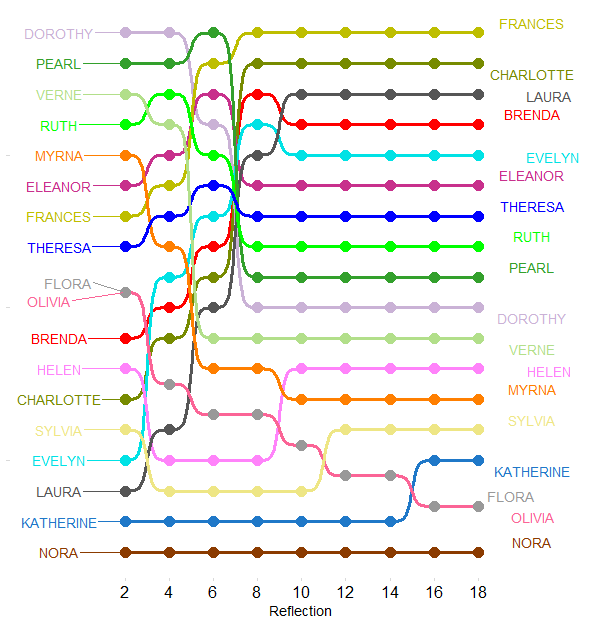
\includegraphics{Plots/p-reflections-sw.png}

}

\caption{Person Reflection Trajectories}

\end{figure}
\end{column}

\begin{column}{0.5\textwidth}
\begin{figure}

{\centering 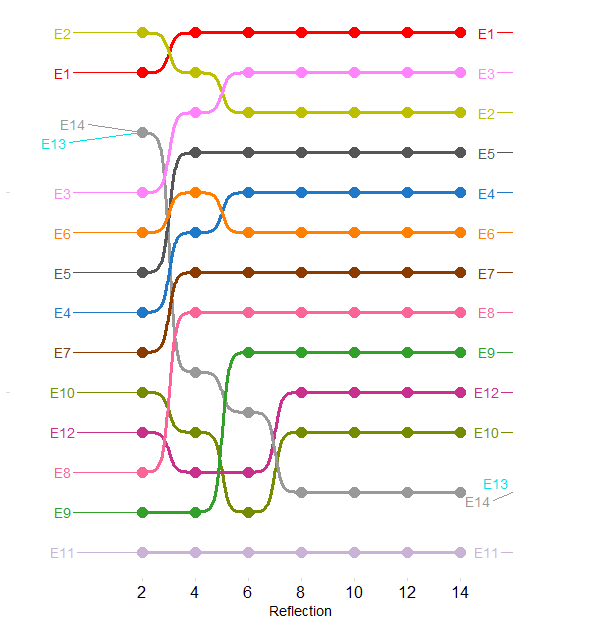
\includegraphics{Plots/g-reflections-sw.png}

}

\caption{Group Reflection Trajectories}

\end{figure}
\end{column}
\end{columns}
\end{frame}

\begin{frame}{Final Reflection Ordering versus CA}
\protect\hypertarget{final-reflection-ordering-versus-ca}{}
\begin{columns}[T]
\begin{column}{0.5\textwidth}
\begin{figure}

{\centering 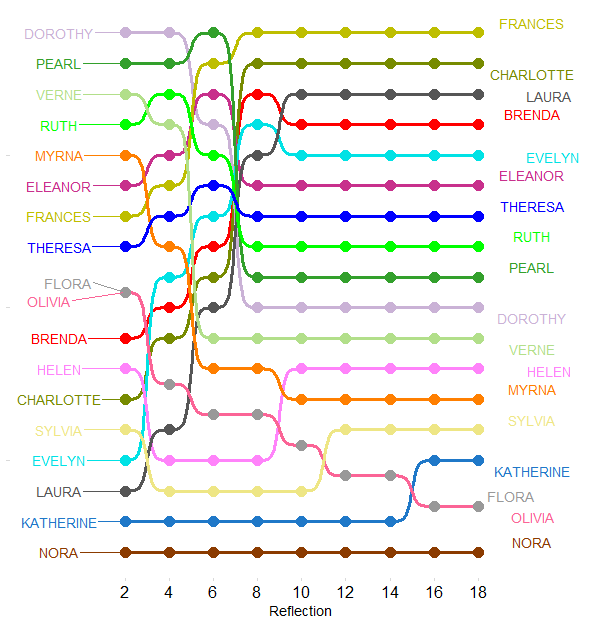
\includegraphics{Plots/p-reflections-sw.png}

}

\caption{Person Reflection Trajectories}

\end{figure}
\end{column}

\begin{column}{0.5\textwidth}
\begin{figure}

{\centering 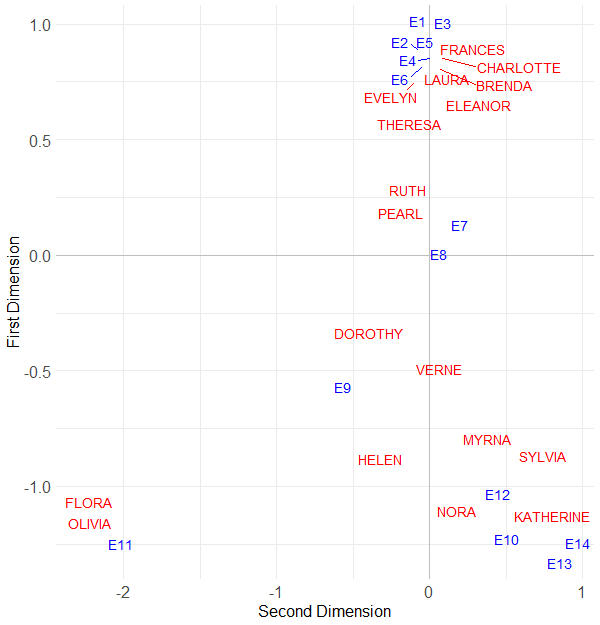
\includegraphics{Plots/ca-sw.png}

}

\caption{Correspondence Plot of Southern Women Data}

\end{figure}
\end{column}
\end{columns}
\end{frame}

\begin{frame}{Final Reflection Ordering versus CA}
\protect\hypertarget{final-reflection-ordering-versus-ca-1}{}
\begin{columns}[T]
\begin{column}{0.5\textwidth}
\begin{figure}

{\centering 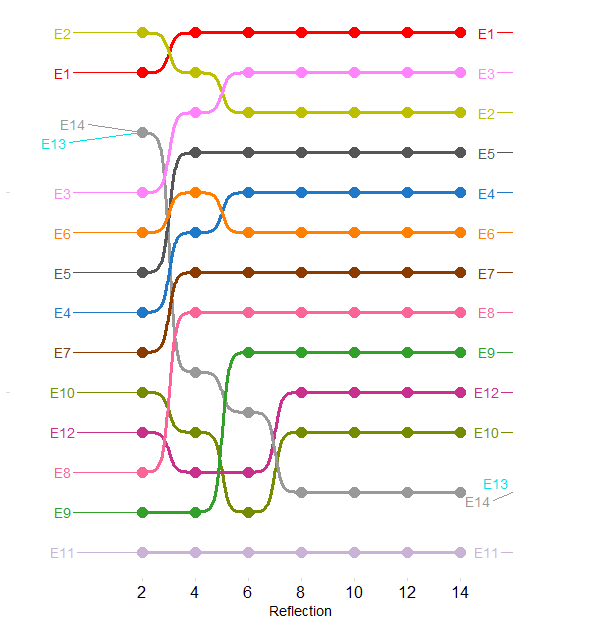
\includegraphics{Plots/g-reflections-sw.png}

}

\caption{Person Reflection Trajectories}

\end{figure}
\end{column}

\begin{column}{0.5\textwidth}
\begin{figure}

{\centering 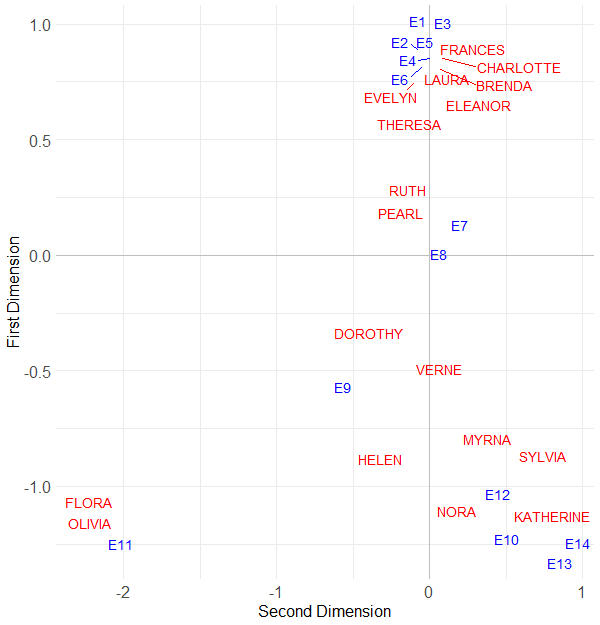
\includegraphics{Plots/ca-sw.png}

}

\caption{Correspondence Plot of Southern Women Data}

\end{figure}
\end{column}
\end{columns}
\end{frame}

\begin{frame}{Final Reflection Ordering versus CA}
\protect\hypertarget{final-reflection-ordering-versus-ca-2}{}
\begin{columns}[T]
\begin{column}{0.5\textwidth}
\begin{figure}

{\centering 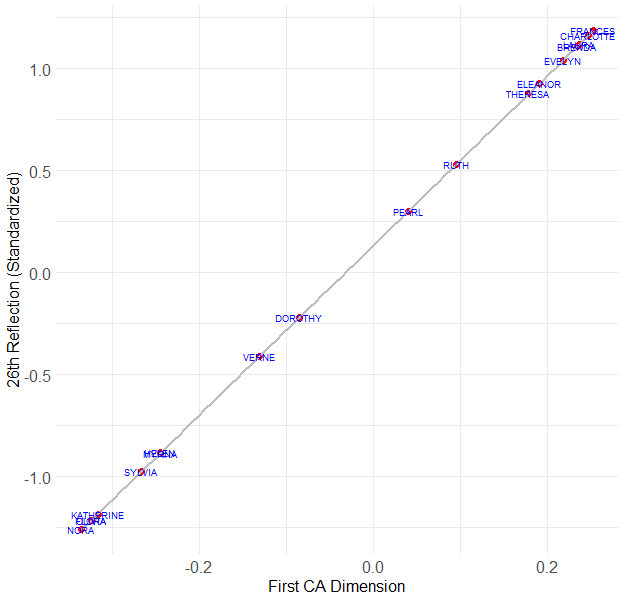
\includegraphics{Plots/p-ca-ref-corr-sw.png}

}

\caption{Scatter of standardized person reflection centralities and
person scores on first CA dimension (r = 1.0)}

\end{figure}
\end{column}

\begin{column}{0.5\textwidth}
\begin{figure}

{\centering 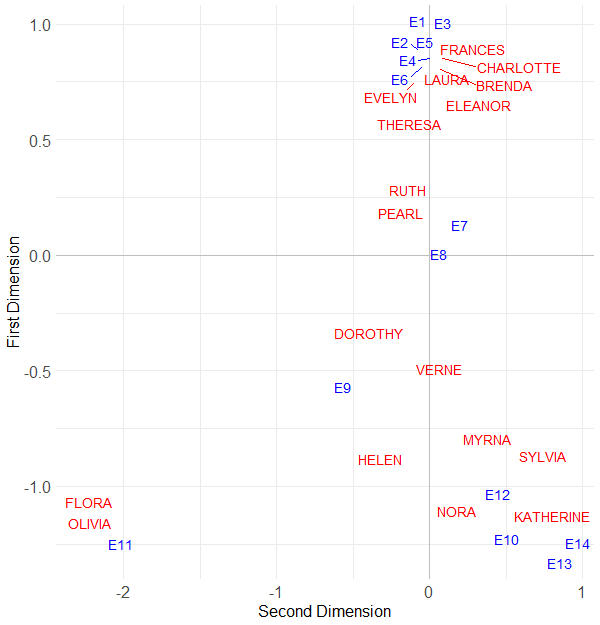
\includegraphics{Plots/ca-sw.png}

}

\caption{Correspondence Plot of Southern Women Data}

\end{figure}
\end{column}
\end{columns}
\end{frame}

\begin{frame}{Final Reflection Ordering versus CA}
\protect\hypertarget{final-reflection-ordering-versus-ca-3}{}
\begin{columns}[T]
\begin{column}{0.5\textwidth}
\begin{figure}

{\centering 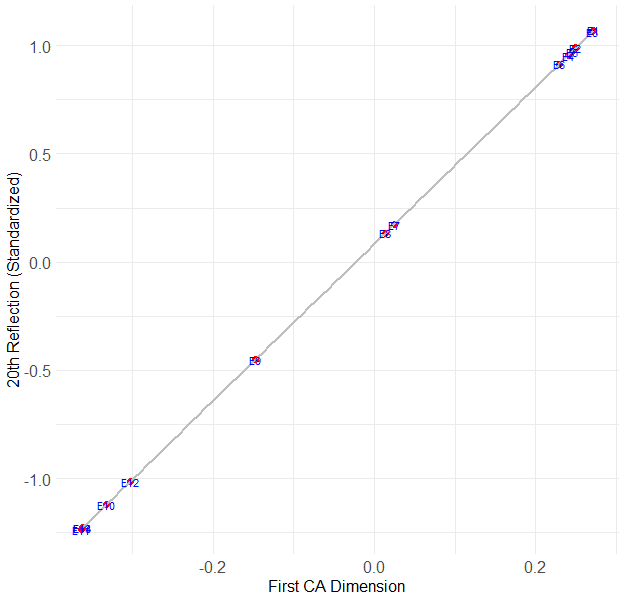
\includegraphics{Plots/g-ca-ref-corr-sw.png}

}

\caption{Scatter of standardized group reflection centralities and group
scores on first CA dimension (r = 1.0)}

\end{figure}
\end{column}

\begin{column}{0.5\textwidth}
\begin{figure}

{\centering 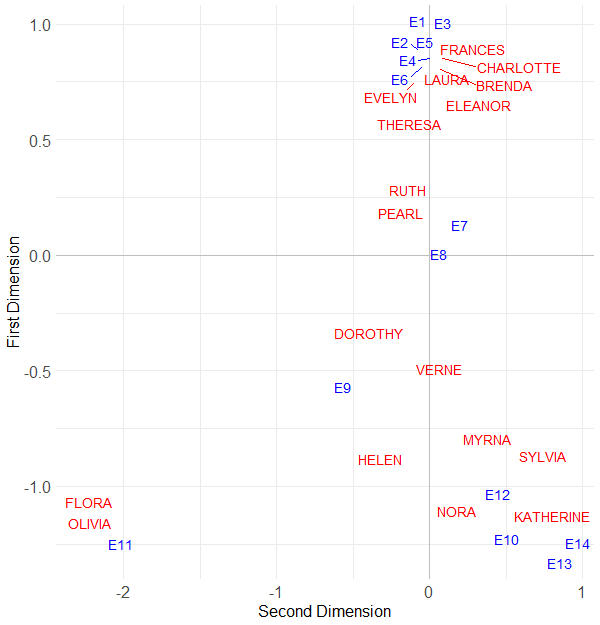
\includegraphics{Plots/ca-sw.png}

}

\caption{Correspondence Plot of Southern Women Data}

\end{figure}
\end{column}
\end{columns}
\end{frame}

\begin{frame}{Method of Reflections versus CA}
\protect\hypertarget{method-of-reflections-versus-ca}{}
\begin{itemize}
\item
  So the method of reflections is an accidental re-invention of CA!*
\item
  But \emph{why} is it a reinvention of CA?

  \begin{itemize}
  \tightlist
  \item
    Short answer:

    \begin{itemize}
    \tightlist
    \item
      The final reflection scores are the (second largest) eigenvalues
      of a matrix, just like CA!
    \end{itemize}
  \end{itemize}
\item
  What's the (slightly) longer answer?

  \begin{itemize}
  \tightlist
  \item
    A couple of things first:

    \begin{itemize}
    \tightlist
    \item
      \(Dp\) is a \(|P| \times |P|\) square degree matrix containing
      each person's \(C_p^R(1)\) (activity) along the diagonals and
      zeroes in every other cell
    \item
      \(Dg\) is a \(|G| \times |G|\) square degree matrix containing
      each group's \(C_g^R(1)\) (size) along the diagonals and zeroes in
      every other cell
    \end{itemize}
  \end{itemize}
\end{itemize}

\marginnote{\begin{footnotesize}

*On the first dimension: Mealy 2019; van Dam et al.~2021

\end{footnotesize}}
\end{frame}

\begin{frame}{Method of Reflections versus CA}
\protect\hypertarget{method-of-reflections-versus-ca-1}{}
\begin{itemize}
\item
  So the method of reflections is an accidental re-invention of CA!*
\item
  But \emph{why} is it a reinvention of CA?

  \begin{itemize}
  \tightlist
  \item
    Short answer:

    \begin{itemize}
    \tightlist
    \item
      The final reflection scores are the (second largest) eigenvalues
      of a matrix, just like CA!
    \end{itemize}
  \end{itemize}
\item
  What's the (slightly) longer answer?

  \begin{itemize}
  \tightlist
  \item
    In the limit (\(q \rightarrow \infty\)), the iterative
    Hidalgo-Hausmann reflective centralities are the solution of the
    eigensystem:*
  \end{itemize}
\end{itemize}

\begin{equation}\protect\hypertarget{eq-dam1}{}{
\left(Dp^{-1}ADg^{-1}A^T\right)C^R_p = \lambda C^R_p
}\label{eq-dam1}\end{equation}

\begin{equation}\protect\hypertarget{eq-dam2}{}{
\left(Dg^{-1}A^TDp^{-1}A\right)C^R_g = \lambda C^R_g
}\label{eq-dam2}\end{equation}

\marginnote{\begin{footnotesize}

*van Dam et al.~2021

\end{footnotesize}}
\end{frame}

\begin{frame}{CA versus Bonacich}
\protect\hypertarget{ca-versus-bonacich}{}
\begin{itemize}
\tightlist
\item
  Do the matrices whose eigenvalues yield the equilibrium reflective
  centralities look familiar to you?
\end{itemize}

\[
\left(Dp^{-1}ADg^{-1}A^T\right)C^R_p = \lambda C^R_p
\]

\[
\left(Dg^{-1}A^TDp^{-1}A\right)C^R_g = \lambda C^R_g
\]

\begin{itemize}
\tightlist
\item
  They should, because the solutions to the following eigensystem give
  the Bonacich \((C^B)\) dual centralities for two-mode networks:*
\end{itemize}

\begin{equation}\protect\hypertarget{eq-bon1}{}{
\left(AA^T\right)C^B_p = \lambda C^B_p
}\label{eq-bon1}\end{equation}

\begin{equation}\protect\hypertarget{eq-bon2}{}{
\left(A^TA\right)C^B_g = \lambda C^B_g
}\label{eq-bon2}\end{equation}

\marginnote{\begin{footnotesize}

*Bonacich 1991

\end{footnotesize}}
\end{frame}

\begin{frame}{CA versus Bonacich}
\protect\hypertarget{ca-versus-bonacich-1}{}
\begin{itemize}
\tightlist
\item
  So both Reflective and Bonacich centralities are eigenvectors of the
  person and group \textbf{projections} of the two-mode network
\end{itemize}

\[
\left(Dp^{-1}ADg^{-1}A^T\right)C^R_p = \lambda C^R_p
\\
\left(Dg^{-1}A^TDp^{-1}A\right)C^R_g = \lambda C^R_g
\\
\left(AA^T\right)C^B_p = \lambda C^B_p
\\
\left(A^TA\right)C^B_g = \lambda C^B_g
\]

\begin{itemize}
\tightlist
\item
  But for reflective centralities the affiliation matrix and its
  transpose are pre-multiplied by the \textbf{inverse of the degree
  matrix of each mode}*
\end{itemize}

\marginnote{\begin{footnotesize}

\begin{itemize}
\tightlist
\item
  van Dam et al.~2021
\end{itemize}

\end{footnotesize}}
\end{frame}

\begin{frame}{CA versus Bonacich}
\protect\hypertarget{ca-versus-bonacich-2}{}
\begin{itemize}
\tightlist
\item
  So both Reflective and Bonacich centralities are eigenvectors of the
  person and group \textbf{projections} of the two-mode network
\end{itemize}

\[
\left(Dp^{-1}ADg^{-1}A^T\right)C^R_p = \lambda C^R_p
\\
\left(Dg^{-1}A^TDp^{-1}A\right)C^R_g = \lambda C^R_g
\\
\left(AA^T\right)C^B_p = \lambda C^B_p
\\
\left(A^TA\right)C^B_g = \lambda C^B_g
\]

\begin{itemize}
\tightlist
\item
  Similar to how each entry in the original affiliation matrix is
  weighted in CA performing the SVD!*
\end{itemize}

\[
Dp^{-1/2}ADg^{-1/2} = X_p \lambda X_g^T
\]

\marginnote{\begin{footnotesize}

**Faust 2005, eq. 7.8

\end{footnotesize}}
\end{frame}

\begin{frame}{CA versus Bonacich}
\protect\hypertarget{ca-versus-bonacich-3}{}
\begin{itemize}
\tightlist
\item
  We can gain some insight into the equivalence between CA and
  Reflections by expressing the degree-weighted projections in terms of
  each cell entry:*
\end{itemize}

\begin{equation}\protect\hypertarget{eq-mealy1}{}{
a_{pp'} = \sum_g\frac{a_{pg}a_{p'g}}{C^R_p(1)C^R_g(1)} = 
    \frac{1}{C^R_p}\sum_g\frac{a_{pg}a_{p'g}}{C^R_g(1)}
}\label{eq-mealy1}\end{equation}

\begin{itemize}
\item
  In Equation~\ref{eq-mealy1}, the fraction's numerator is equal to one
  only when person \(p\) and \(p'\) are both members of \(g\).

  \begin{itemize}
  \tightlist
  \item
    Summed across groups, this is the number of \textbf{shared groups}
    between \(p\) and \(p'\):

    \begin{itemize}
    \tightlist
    \item
      The cell entries in the Bonacich matrix (raw projections)
    \end{itemize}
  \item
    But in Equation~\ref{eq-mealy1} the numerator is \emph{weighted} by
    the product of group size and each person's number of memberships
    (in contrast to Bonacich)
  \end{itemize}
\end{itemize}

\marginnote{\begin{footnotesize}

*Mealy 2019, eq. 4

\end{footnotesize}}
\end{frame}

\begin{frame}{CA versus Bonacich}
\protect\hypertarget{ca-versus-bonacich-4}{}
\begin{itemize}
\tightlist
\item
  We can gain some insight into the equivalence between CA and
  Reflections by expressing the degree-weighted projections in terms of
  each cell entry:*
\end{itemize}

\begin{equation}\protect\hypertarget{eq-mealy2}{}{
    a_{gg'} = \sum_p\frac{a_{pg}a_{pg'}}{C^R_p(1)C^R_g(1)} = 
    \frac{1}{C^R_g}\sum_p\frac{a_{pg}a_{pg'}}{C^R_p(1)}
}\label{eq-mealy2}\end{equation}

\begin{itemize}
\item
  In Equation~\ref{eq-mealy2}, the fraction's numerator is equal to one
  only when group \(g\) and \(g'\) both have \(p\) as a member

  \begin{itemize}
  \tightlist
  \item
    Summed across persons, the number of \textbf{shared members} between
    \(g\) and \(g'\):

    \begin{itemize}
    \tightlist
    \item
      The cell entries in the Bonacich matrix (raw projections)
    \end{itemize}
  \item
    But in Equation~\ref{eq-mealy2} the numerator is \emph{weighted} by
    the product of group size and each person's number of memberships
    (in contrast to Bonacich)
  \end{itemize}
\end{itemize}

\marginnote{\begin{footnotesize}

*Mealy 2019, eq. 4

\end{footnotesize}}
\end{frame}

\begin{frame}{CA versus Bonacich}
\protect\hypertarget{ca-versus-bonacich-5}{}
\begin{columns}[T]
\begin{column}{0.5\textwidth}
\begin{figure}

{\centering 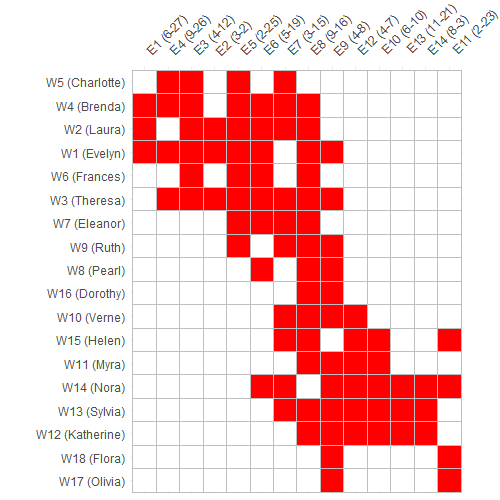
\includegraphics{Plots/ca-reord.png}

}

\caption{CA Re-ordered Affiliation Matrix}

\end{figure}
\end{column}

\begin{column}{0.5\textwidth}
\begin{figure}

{\centering 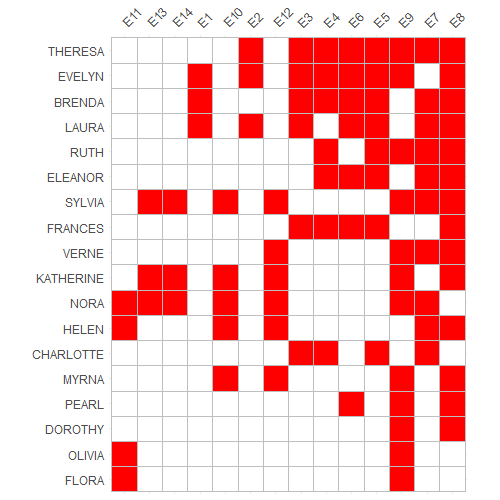
\includegraphics{Plots/bon-reord.png}

}

\caption{Bonacich Re-ordered Affiliation Matrix}

\end{figure}
\end{column}
\end{columns}
\end{frame}

\begin{frame}{CA versus Bonacich}
\protect\hypertarget{ca-versus-bonacich-6}{}
\begin{columns}[T]
\begin{column}{0.5\textwidth}
\begin{figure}

{\centering 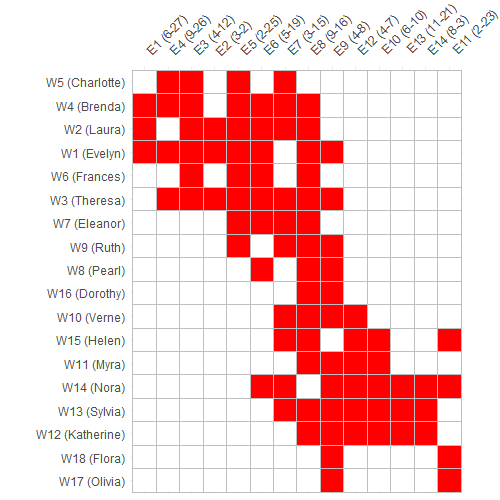
\includegraphics{Plots/ca-reord.png}

}

\caption{CA Re-ordered Affiliation Matrix}

\end{figure}
\end{column}

\begin{column}{0.5\textwidth}
\begin{itemize}
\tightlist
\item
  The CA re-ordered affiliation matrix is \textbf{block-diagonal}
\item
  Reveals (a well-known and storied*) grouping of persons and groups
  into two clusters 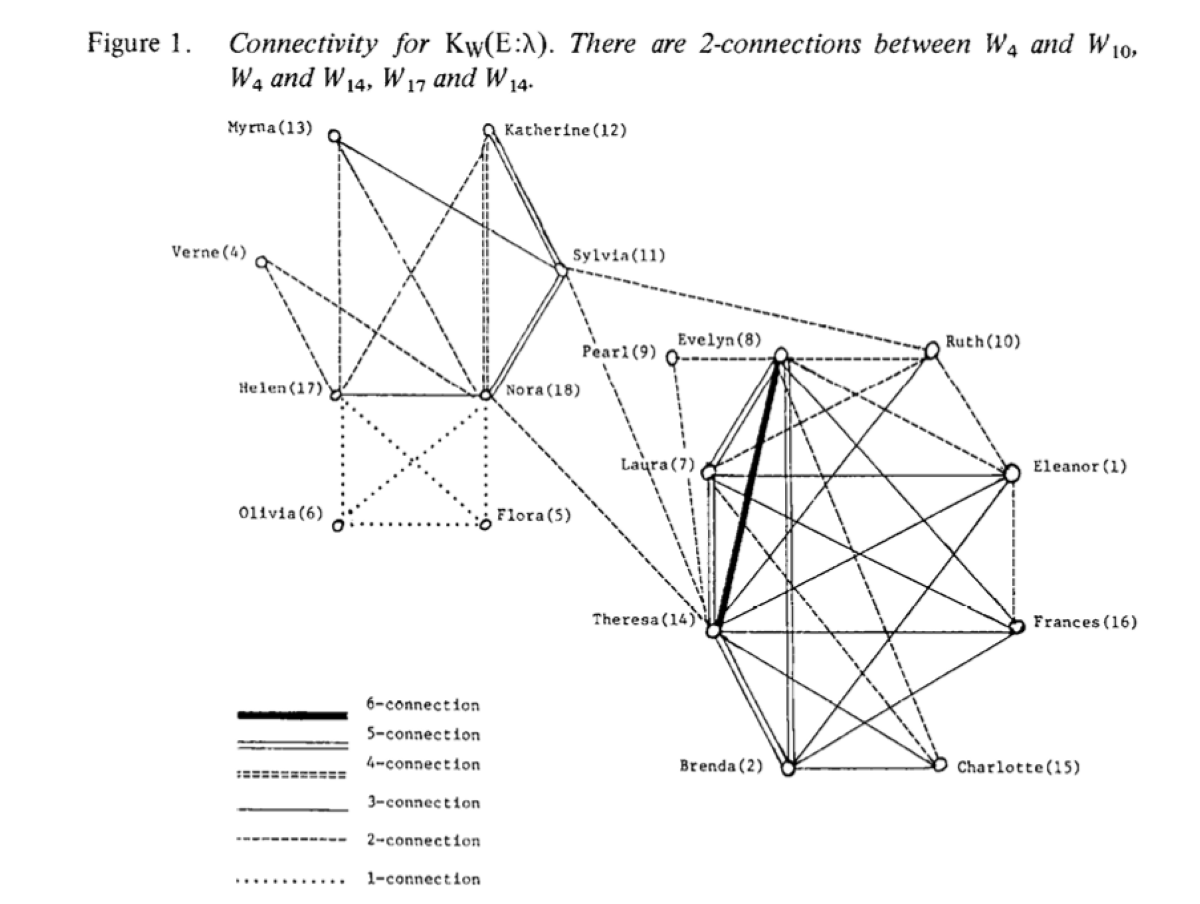
\includegraphics{Plots/doreian-sw.png}
\end{itemize}
\end{column}
\end{columns}
\end{frame}

\begin{frame}{CA versus Bonacich}
\protect\hypertarget{ca-versus-bonacich-7}{}
\begin{columns}[T]
\begin{column}{0.5\textwidth}
\begin{figure}

{\centering 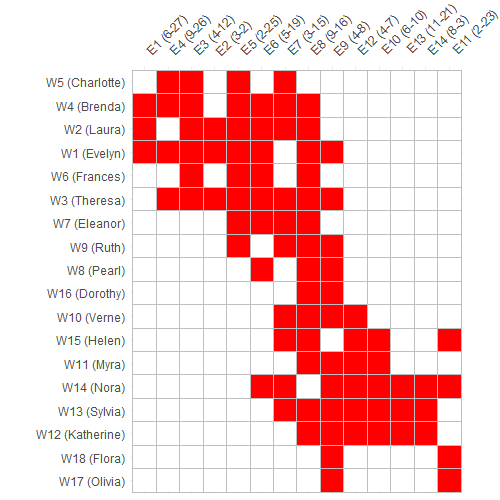
\includegraphics{Plots/ca-reord.png}

}

\caption{CA Re-ordered Affiliation Matrix}

\end{figure}
\end{column}

\begin{column}{0.5\textwidth}
\begin{itemize}
\tightlist
\item
  First CA dimension is also an \textbf{ordering} so it counts as a
  centrality (a rank over the nodes)
\item
  It is an ordering that uses a logic of grouping in order to rank

  \begin{itemize}
  \tightlist
  \item
    Tasks usually segregated in sna
  \end{itemize}
\item
  Central events contain the most central people and central people
  attend the most central events:

  \begin{itemize}
  \tightlist
  \item
    \(E1 = \{Laura, Brenda, Evelyn\}\)
  \end{itemize}
\item
  In CA ordering central events are \emph{not} the ones with most
  members!

  \begin{itemize}
  \tightlist
  \item
    \(\{E7, E8, E9\}\)
  \end{itemize}
\end{itemize}
\end{column}
\end{columns}
\end{frame}

\begin{frame}{CA versus Bonacich}
\protect\hypertarget{ca-versus-bonacich-8}{}
\begin{columns}[T]
\begin{column}{0.5\textwidth}
\begin{figure}

{\centering 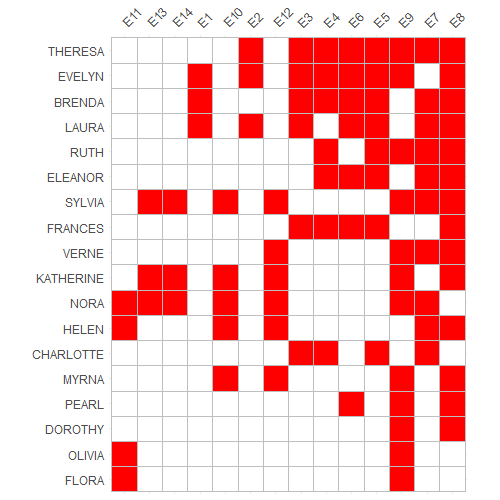
\includegraphics{Plots/bon-reord.png}

}

\caption{CA Re-ordered Affiliation Matrix}

\end{figure}
\end{column}

\begin{column}{0.5\textwidth}
\begin{itemize}
\tightlist
\item
  First CA dimension is also an \textbf{ordering} so it counts as a
  centrality (a rank over the nodes)
\item
  It is an ordering that uses a logic of grouping in order to rank

  \begin{itemize}
  \tightlist
  \item
    Tasks usually segregated in sna
  \end{itemize}
\item
  Central events contain the most central people and central people
  attend the most central events:

  \begin{itemize}
  \tightlist
  \item
    \(E1 = \{Laura, Brenda, Evelyn\}\)
  \end{itemize}
\item
  But they are the most central in the Bonacich ordering!

  \begin{itemize}
  \tightlist
  \item
    \(\{E7, E8, E9\}\)
  \end{itemize}
\end{itemize}
\end{column}
\end{columns}
\end{frame}

\begin{frame}{CA versus Bonacich}
\protect\hypertarget{ca-versus-bonacich-9}{}
\begin{columns}[T]
\begin{column}{0.5\textwidth}
\begin{figure}

{\centering 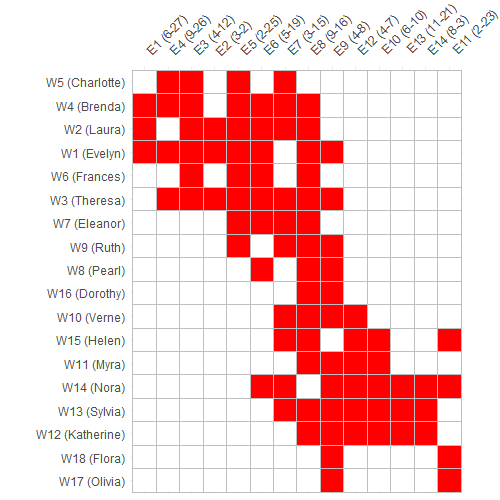
\includegraphics{Plots/ca-reord.png}

}

\caption{CA Re-ordered Affiliation Matrix}

\end{figure}
\end{column}

\begin{column}{0.5\textwidth}
\begin{itemize}
\tightlist
\item
  First CA dimension is also an \textbf{ordering} so it counts as a
  centrality (a rank over the nodes)
\item
  It is an ordering that uses a logic of grouping in order to rank

  \begin{itemize}
  \tightlist
  \item
    Tasks usually segregated in sna
  \end{itemize}
\item
  Least central events contain many of the least central people:

  \begin{itemize}
  \tightlist
  \item
    \(E11 = \{Helen, Flora, Olivia, \\ Nora\}\)
  \end{itemize}
\item
  In CA ordering less central events are \emph{not} the ones with the
  least members!

  \begin{itemize}
  \tightlist
  \item
    \(\{E1, E13, E14\}\)
  \item
    \(E1\) is the most central!
  \end{itemize}
\end{itemize}
\end{column}
\end{columns}
\end{frame}

\begin{frame}{CA versus Bonacich}
\protect\hypertarget{ca-versus-bonacich-10}{}
\begin{columns}[T]
\begin{column}{0.5\textwidth}
\begin{figure}

{\centering 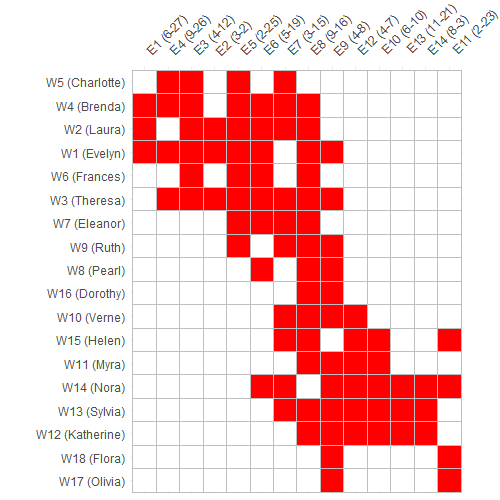
\includegraphics{Plots/ca-reord.png}

}

\caption{CA Re-ordered Affiliation Matrix}

\end{figure}
\end{column}

\begin{column}{0.5\textwidth}
\begin{itemize}
\tightlist
\item
  First CA dimension is also an \textbf{ordering} so it counts as a
  centrality (a rank over the nodes)
\item
  It is an ordering that uses a logic of grouping in order to rank

  \begin{itemize}
  \tightlist
  \item
    Tasks usually segregated in sna
  \end{itemize}
\item
  Central people attend the most central events and central events are
  attended by central people:

  \begin{itemize}
  \tightlist
  \item
    \(Frances = \{E3, E5, E4, E6, E8\}\)
  \end{itemize}
\item
  Not necessarily those with the most memberships

  \begin{itemize}
  \tightlist
  \item
    \(\{Theresa, Evelyn, Brenda\}\)
  \end{itemize}
\end{itemize}
\end{column}
\end{columns}
\end{frame}

\begin{frame}{CA versus Bonacich}
\protect\hypertarget{ca-versus-bonacich-11}{}
\begin{columns}[T]
\begin{column}{0.5\textwidth}
\begin{figure}

{\centering 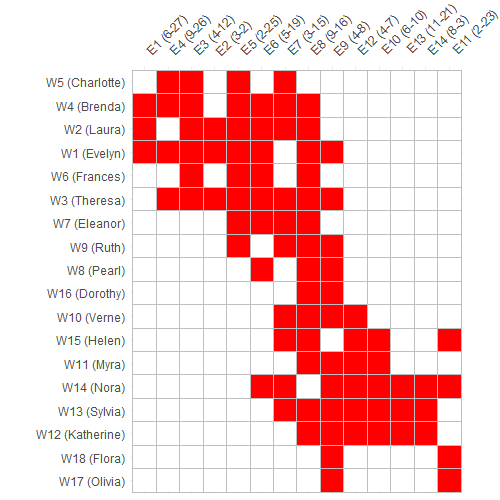
\includegraphics{Plots/ca-reord.png}

}

\caption{CA Re-ordered Affiliation Matrix}

\end{figure}
\end{column}

\begin{column}{0.5\textwidth}
\begin{itemize}
\tightlist
\item
  First CA dimension is also an \textbf{ordering} so it counts as a
  centrality (a rank over the nodes)
\item
  It is an ordering that uses a logic of grouping in order to rank

  \begin{itemize}
  \tightlist
  \item
    Tasks usually segregated in sna
  \end{itemize}
\item
  The least central person \(\{Nora\}\) is not the one with the least
  memberships

  \begin{itemize}
  \tightlist
  \item
    Instead \(\{Nora\}\) shares many memberships with less central
    people (those who attend the less central events)
  \item
    \(\{Flora, Olivia, Sylvia, Kat.\}\)
  \end{itemize}
\end{itemize}
\end{column}
\end{columns}
\end{frame}

\begin{frame}{CA versus Bonacich}
\protect\hypertarget{ca-versus-bonacich-12}{}
\begin{columns}[T]
\begin{column}{0.5\textwidth}
\begin{figure}

{\centering 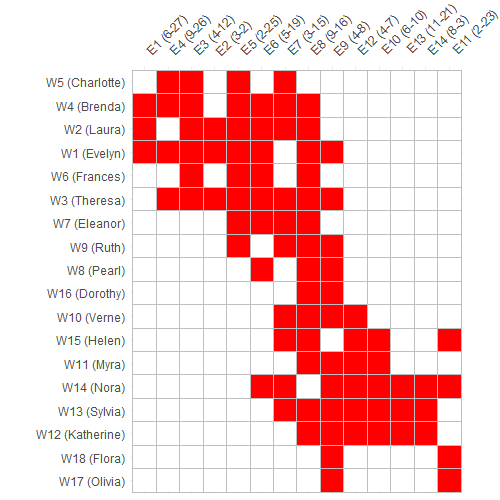
\includegraphics{Plots/ca-reord.png}

}

\caption{CA Re-ordered Affiliation Matrix}

\end{figure}
\end{column}

\begin{column}{0.5\textwidth}
\begin{itemize}
\tightlist
\item
  First CA dimension is also an \textbf{ordering} so it counts as a
  centrality (a rank over the nodes)
\item
  It is an ordering that uses a logic of grouping in order to rank

  \begin{itemize}
  \tightlist
  \item
    Tasks usually segregated in sna
  \end{itemize}
\item
  Central people attend the most central events and central events are
  attended by central people:

  \begin{itemize}
  \tightlist
  \item
    \(E1 = \{Laura, Brenda, Evelyn\}\)
  \end{itemize}
\item
  In CA ordering central events are \emph{not} the ones with the most
  members!

  \begin{itemize}
  \tightlist
  \item
    e.g., \(\{E7, E8, E9\}\)
  \end{itemize}
\end{itemize}
\end{column}
\end{columns}
\end{frame}

\begin{frame}{CA versus Bonacich}
\protect\hypertarget{ca-versus-bonacich-13}{}
\begin{columns}[T]
\begin{column}{0.5\textwidth}
\begin{figure}

{\centering 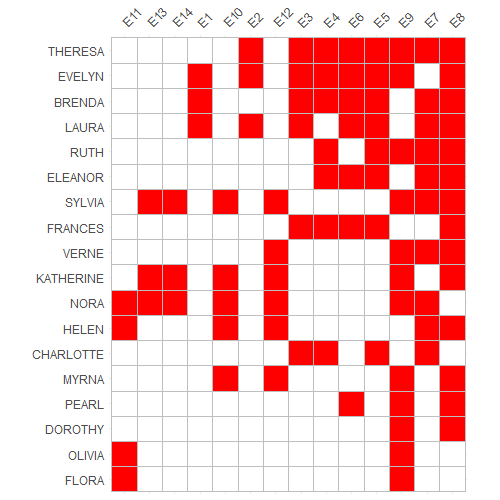
\includegraphics{Plots/bon-reord.png}

}

\caption{Bonacich Re-ordered Affiliation Matrix}

\end{figure}
\end{column}

\begin{column}{0.5\textwidth}
\begin{itemize}
\tightlist
\item
  The Bonacich re-ordered affiliation matrix is \textbf{upper
  triangular}
\item
  Arranges persons and groups from top to bottom and left to right by
  activity and size respectively

  \begin{itemize}
  \tightlist
  \item
    More central people and groups at the upper right
  \item
    Less central people and groups at the lower left
  \end{itemize}
\end{itemize}
\end{column}
\end{columns}
\end{frame}

\begin{frame}{CA versus Bonacich}
\protect\hypertarget{ca-versus-bonacich-14}{}
\begin{columns}[T]
\begin{column}{0.5\textwidth}
\begin{figure}

{\centering 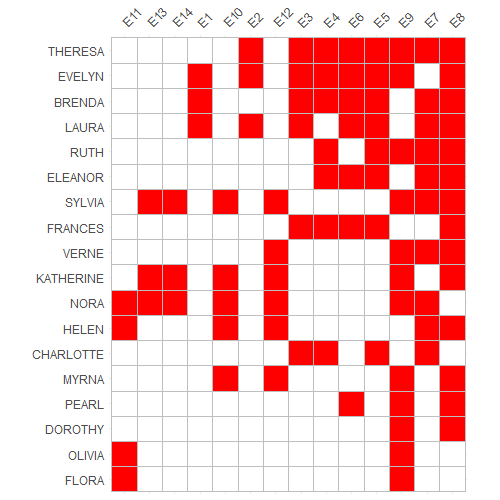
\includegraphics{Plots/bon-reord.png}

}

\caption{Bonacich Re-ordered Affiliation Matrix}

\end{figure}
\end{column}

\begin{column}{0.5\textwidth}
\begin{itemize}
\tightlist
\item
  Bonacich centrality is dual but it is ``simple'' dual

  \begin{itemize}
  \tightlist
  \item
    Central people attend well-attended events
  \item
    Central events are attended by people who attend many events
  \end{itemize}
\item
  Centrality in one mode is a weighted \emph{sum} of the other mode's
  centrality*
\end{itemize}

\begin{equation}\protect\hypertarget{eq-fau1}{}{
    C^B_p = \frac{1}{\lambda}\sum_{g}a_{pg}C^B_g
}\label{eq-fau1}\end{equation}

\begin{equation}\protect\hypertarget{eq-fau2}{}{
    C^B_g = \frac{1}{\lambda}\sum_{p}a_{pg}C^B_p
}\label{eq-fau2}\end{equation}
\end{column}
\end{columns}

\marginnote{\begin{footnotesize}

*Faust 1997, p.~170

\end{footnotesize}}
\end{frame}

\begin{frame}{CA versus Bonacich}
\protect\hypertarget{ca-versus-bonacich-15}{}
\begin{columns}[T]
\begin{column}{0.5\textwidth}
\begin{figure}

{\centering 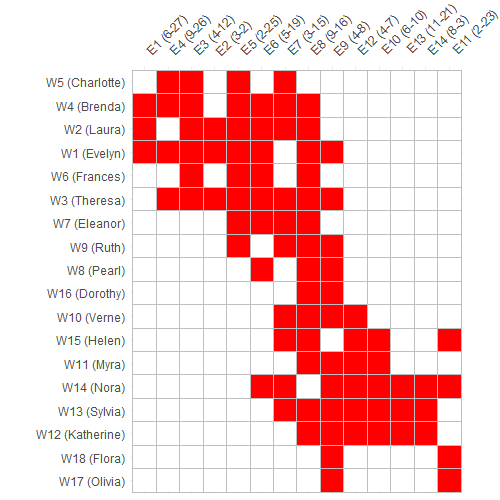
\includegraphics{Plots/ca-reord.png}

}

\caption{CA Re-ordered Affiliation Matrix}

\end{figure}
\end{column}

\begin{column}{0.5\textwidth}
\begin{itemize}
\tightlist
\item
  CA centrality is dual but it is ``generalized similarity'' dual*

  \begin{itemize}
  \tightlist
  \item
    Central people attend central (not necessarily the most
    well-attended) events
  \item
    Central events are attended by central (not necessarily the most
    active) people
  \end{itemize}
\item
  Some people calculate Bonacich centralities when they have this more
  ``generalized similarity'' idea of centrality in mind!

  \begin{itemize}
  \tightlist
  \item
    They should use CA instead
  \end{itemize}
\end{itemize}
\end{column}
\end{columns}

\marginnote{\begin{footnotesize}

*Kovacs 2010; Lizardo 2024

\end{footnotesize}}
\end{frame}

\begin{frame}{CA and Similarity}
\protect\hypertarget{ca-and-similarity}{}
\begin{itemize}
\item
  Another way to gain insight into what CA is doing is by looking at the
  similarity of people and groups in the data
\item
  As we all know,* the usual one mode projections are obtained via:
\end{itemize}

\begin{equation}\protect\hypertarget{eq-brei1}{}{
S_p = AA^T
}\label{eq-brei1}\end{equation}

\begin{equation}\protect\hypertarget{eq-brei1}{}{
S_g = A^TA
}\label{eq-brei1}\end{equation}

\begin{itemize}
\tightlist
\item
  Which can be thought of as \textbf{similarity matrices} based on the
  shared neighbors in the two mode network
\end{itemize}

\marginnote{\begin{footnotesize}

Breiger 1974

\end{footnotesize}}
\end{frame}

\begin{frame}{CA and Similarity}
\protect\hypertarget{ca-and-similarity-1}{}
\begin{itemize}
\item
  Another way to gain insight into what CA is doing is by looking at the
  similarity of people and groups in the data
\item
  But we can also obtain \emph{other-mode degree weighted} versions of
  these similarity matrices*
\end{itemize}

\begin{equation}\protect\hypertarget{eq-dam5}{}{
S^*_p = ADg^{-1}A^T
}\label{eq-dam5}\end{equation}

\begin{equation}\protect\hypertarget{eq-dam6}{}{
S^*_g = A^TDp^{-1}A
}\label{eq-dam6}\end{equation}

\marginnote{\begin{footnotesize}

van Dam et al.~2021

\end{footnotesize}}
\end{frame}

\begin{frame}{CA and Similarity}
\protect\hypertarget{ca-and-similarity-2}{}
\begin{columns}[T]
\begin{column}{0.5\textwidth}
\begin{figure}

{\centering 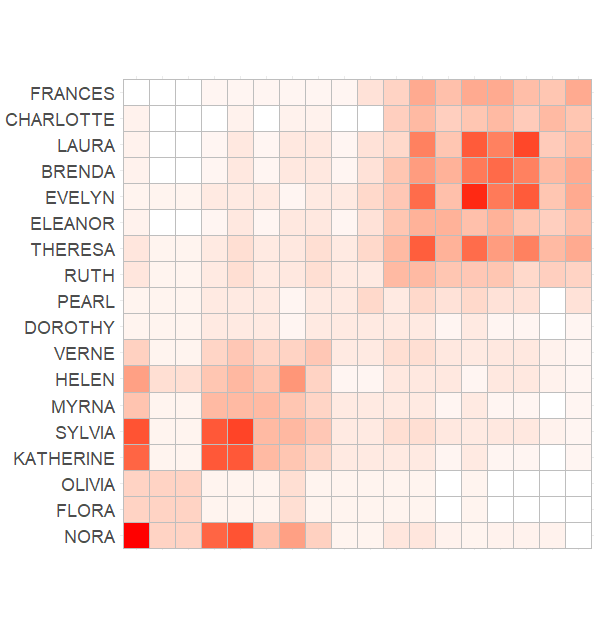
\includegraphics{Plots/ca-sim-p.png}

}

\caption{Degree-weighted similarity matrix (persons)}

\end{figure}
\end{column}

\begin{column}{0.5\textwidth}
\begin{figure}

{\centering 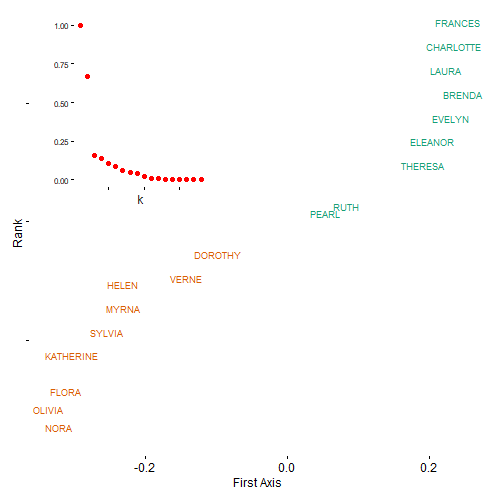
\includegraphics{Plots/ca-eigvec-p.png}

}

\caption{First eigenvalue of person similarity matrix against rank}

\end{figure}
\end{column}
\end{columns}
\end{frame}

\begin{frame}{CA and Similarity}
\protect\hypertarget{ca-and-similarity-3}{}
\begin{columns}[T]
\begin{column}{0.5\textwidth}
\begin{figure}

{\centering 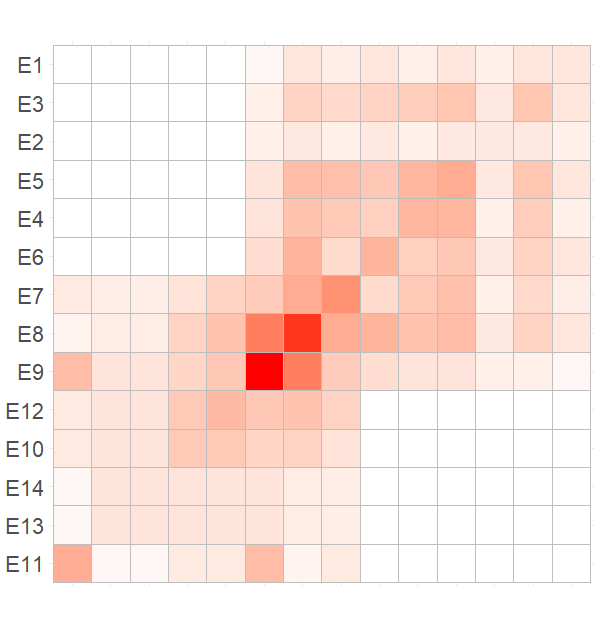
\includegraphics{Plots/ca-sim-g.png}

}

\caption{Degree-weighted similarity matrix (groups)}

\end{figure}
\end{column}

\begin{column}{0.5\textwidth}
\begin{figure}

{\centering 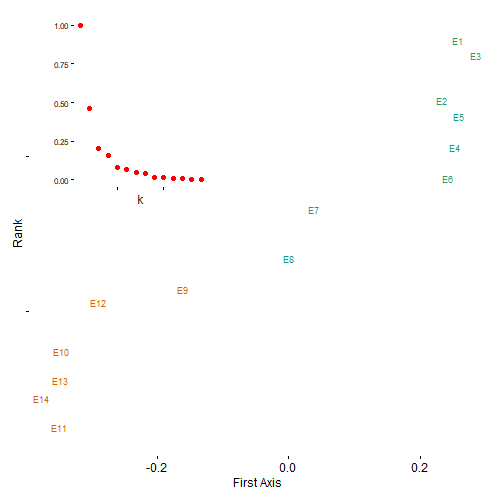
\includegraphics{Plots/ca-eigvec-g.png}

}

\caption{First eigenvalue of group similarity matrix against rank}

\end{figure}
\end{column}
\end{columns}
\end{frame}

\begin{frame}{CA and Similarity}
\protect\hypertarget{ca-and-similarity-4}{}
\begin{columns}[T]
\begin{column}{0.3\textwidth}
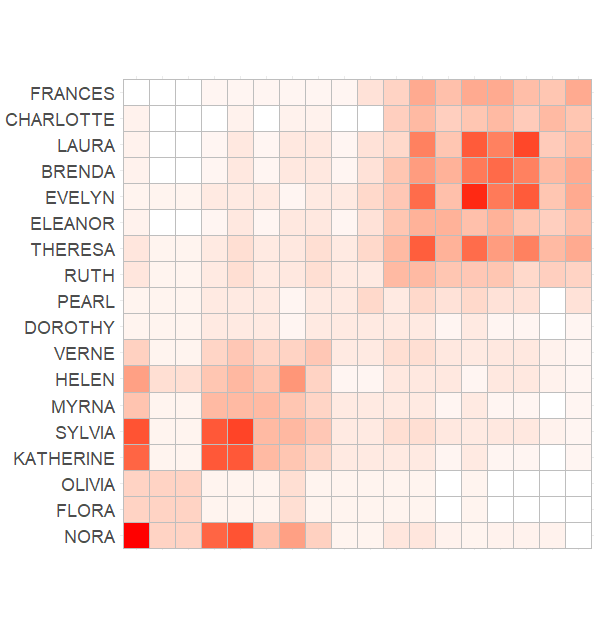
\includegraphics{Plots/ca-sim-p.png}
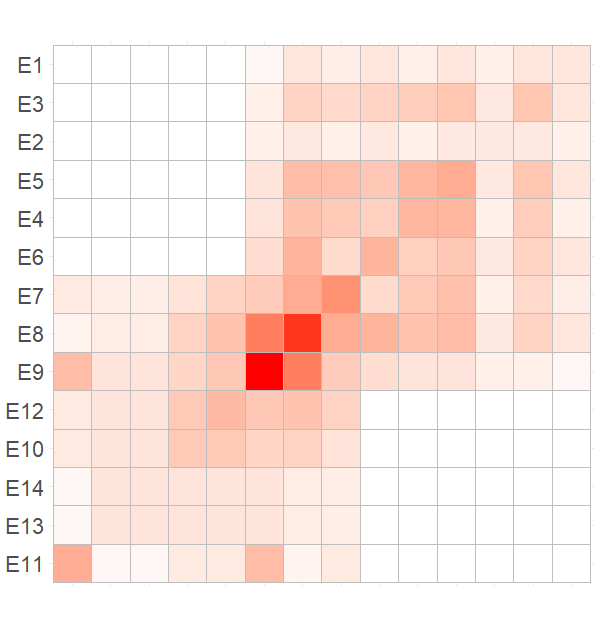
\includegraphics{Plots/ca-sim-g.png}
\end{column}

\begin{column}{0.55\textwidth}
\begin{figure}

{\centering 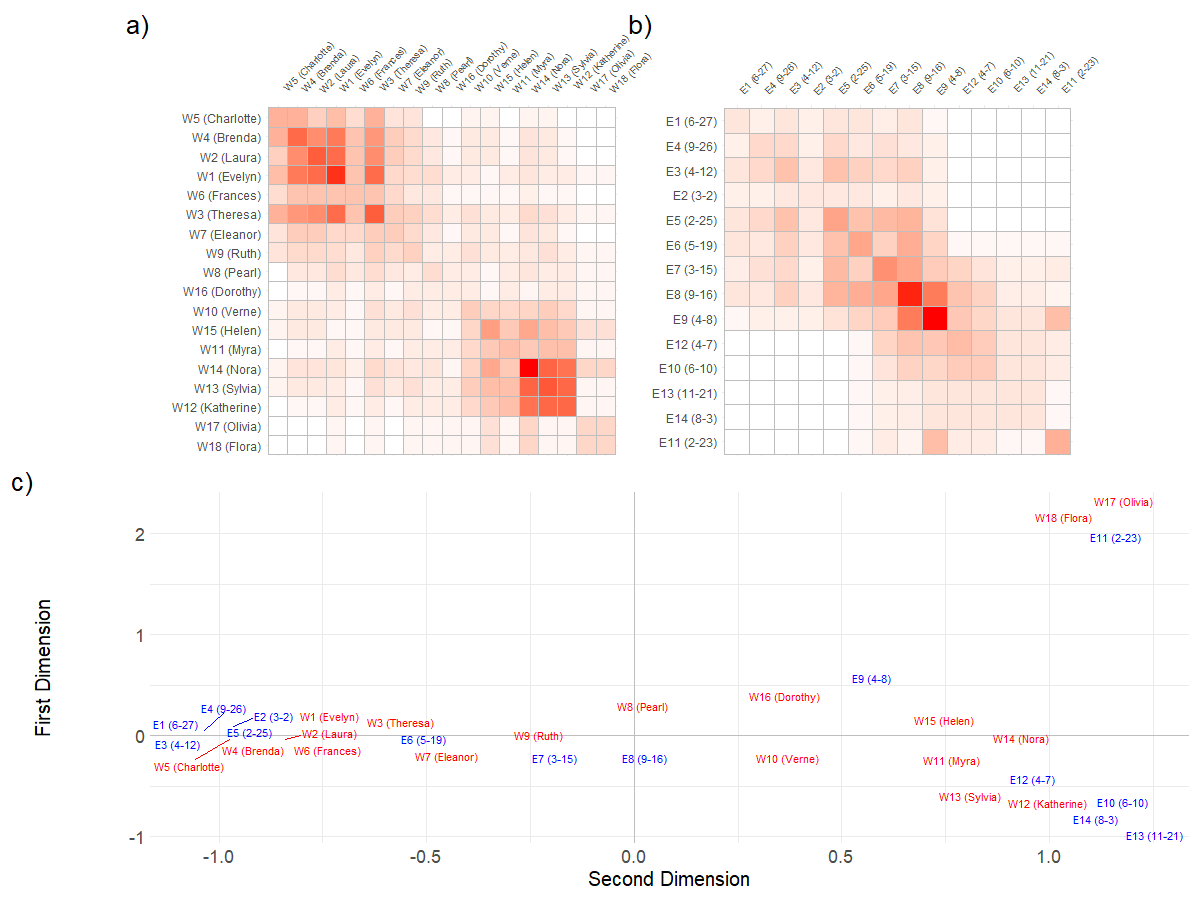
\includegraphics{Plots/ca-corr-plot.png}

}

\caption{CA Correspondence Plot}

\end{figure}
\end{column}
\end{columns}
\end{frame}

\begin{frame}{Bonacich and Similarity}
\protect\hypertarget{bonacich-and-similarity}{}
\begin{columns}[T]
\begin{column}{0.3\textwidth}
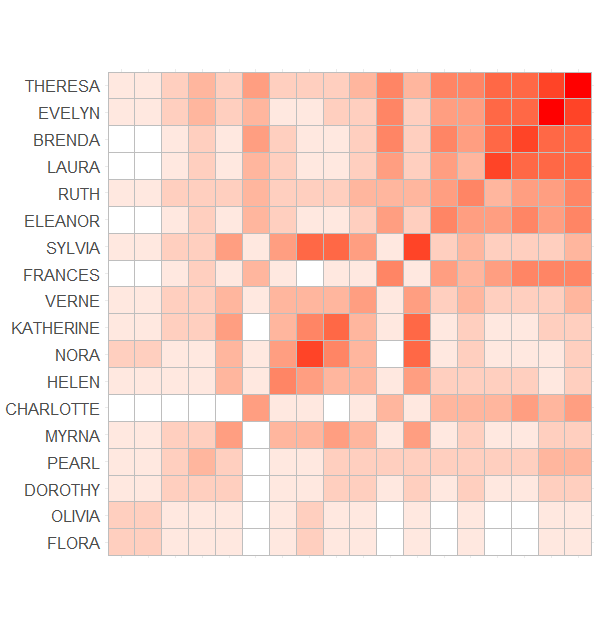
\includegraphics{Plots/bon-sim-p.png}
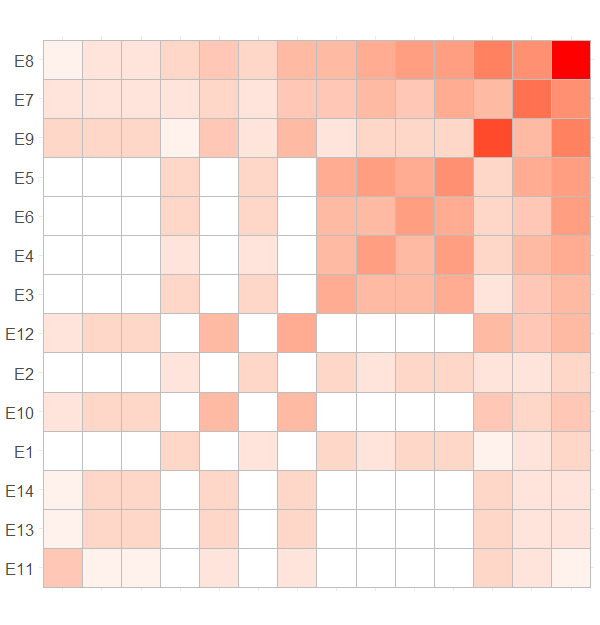
\includegraphics{Plots/bon-sim-g.png}
\end{column}

\begin{column}{0.55\textwidth}
\begin{figure}

{\centering 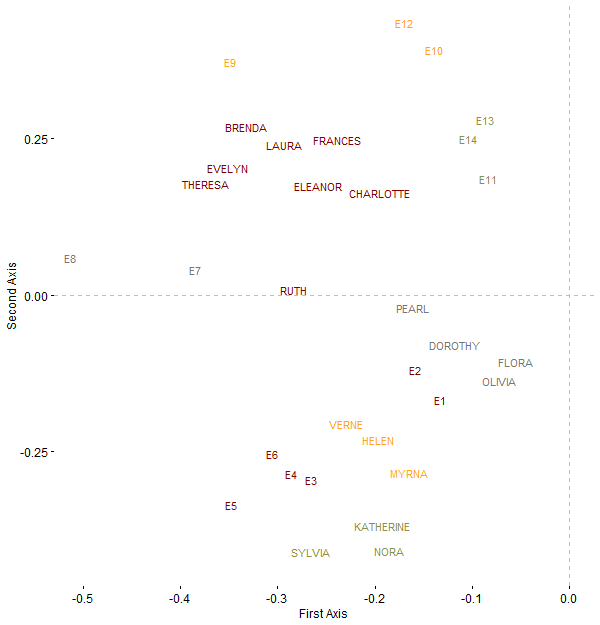
\includegraphics{Plots/bon-corr-plot.png}

}

\caption{Bonacich Correspondence Plot}

\end{figure}
\end{column}
\end{columns}
\end{frame}

\begin{frame}{CA and Generalized Relational Similarity}
\protect\hypertarget{ca-and-generalized-relational-similarity}{}
\begin{itemize}
\tightlist
\item
  Bonacich orders people according to attendance at central (most-well
  attended) events and events according to attendance by central (most
  active) people
\item
  CA orders people according to attendance at \textbf{similarly central
  events} and events according to attendance by \textbf{similarly
  central people}

  \begin{itemize}
  \tightlist
  \item
    This is precisely the definition of \textbf{generalized relational
    similarity} (GSR)*
  \end{itemize}
\end{itemize}

\pause

\begin{itemize}
\tightlist
\item
  In that case proximity of nodes in the first CA dimension may reveal a
  type of GSR in two-mode networks

  \begin{itemize}
  \tightlist
  \item
    Let us see how that works in the case of two candidate two-mode GSRs

    \begin{itemize}
    \tightlist
    \item
      \emph{SimRank} *
    \item
      Similarity Weighted Correlation Distance**
    \end{itemize}
  \end{itemize}
\end{itemize}

\marginnote{\begin{footnotesize}

*Jeh \& Widom 2002

**Kovacs 2010; Lizardo 2024

\end{footnotesize}}
\end{frame}

\begin{frame}{CA and SimRank}
\protect\hypertarget{ca-and-simrank}{}
\begin{itemize}
\tightlist
\item
  To explore the link between CA and GSR we can compare CA with one
  independently developed approach for obtaining GSRs in two-mode
  networks:*

  \begin{itemize}
  \tightlist
  \item
    \emph{SimRank}
  \end{itemize}
\item
  According to \emph{SimRank}:

  \begin{itemize}
  \tightlist
  \item
    People are \emph{similar} if they belong to \emph{similar} groups
  \item
    Groups are \emph{similar} if they share \emph{similar} members
  \end{itemize}
\item
  In \emph{SimRank} the similarity between two people is given by:
\end{itemize}

\begin{equation}\protect\hypertarget{eq-simrank1}{}{
S(p, p') = \frac{\alpha}{C_p^R(1)C_{p'}^R(1)}
    \sum_{i = 1}^{C_p^R(1)} \sum_{j = 1}^{C_{p'}^R(1)} 
    S\left(g(i)_{i \in N(p)}, g(j)_{j \in N(p')}\right)
}\label{eq-simrank1}\end{equation}

\marginnote{\begin{footnotesize}

*Jeh \& Widom 2002

\end{footnotesize}}
\end{frame}

\begin{frame}{CA and SimRank}
\protect\hypertarget{ca-and-simrank-1}{}
\begin{itemize}
\tightlist
\item
  To explore the link between CA and GSR we can compare CA with one
  independently developed approach for obtaining GSRs in two-mode
  networks:*

  \begin{itemize}
  \tightlist
  \item
    \emph{SimRank}
  \end{itemize}
\item
  According to \emph{SimRank}:

  \begin{itemize}
  \tightlist
  \item
    People are \emph{similar} if they belong to \emph{similar} groups
  \item
    Groups are \emph{similar} if they share \emph{similar} members
  \end{itemize}
\item
  In \emph{SimRank} the similarity between two groups is given by:
\end{itemize}

\begin{equation}\protect\hypertarget{eq-simrank2}{}{
S(g, g') = \frac{\alpha}{C_g^R(1)C_{g'}^R(1)}
    \sum_{i = 1}^{C_g^R(1)} \sum_{j = 1}^{C_{g'}^R(1)} 
    S\left(p(i)_{i \in N(g)}, p(j)_{j \in N(g')}\right)
}\label{eq-simrank2}\end{equation}

\marginnote{\begin{footnotesize}

*Jeh \& Widom 2002

\end{footnotesize}}
\end{frame}

\begin{frame}{CA and SimRank}
\protect\hypertarget{ca-and-simrank-2}{}
\begin{itemize}
\tightlist
\item
  \emph{SimRank} for people:
\end{itemize}

\[
\small
S(p, p') = \frac{\alpha}{C_p^R(1)C_{p'}^R(1)}
    \sum_{i = 1}^{C_p^R(1)} \sum_{j = 1}^{C_{p'}^R(1)} 
    S\left(g(i)_{i \in N(p)}, g(j)_{j \in N(p')}\right)
\]

\begin{itemize}
\tightlist
\item
  \emph{SimRank} for groups:
\end{itemize}

\[
\small
S(g, g') = \frac{\alpha}{C_g^R(1)C_{g'}^R(1)}
    \sum_{i = 1}^{C_g^R(1)} \sum_{j = 1}^{C_{g'}^R(1)} 
    S\left(p(i)_{i \in N(g)}, p(j)_{j \in N(g')}\right)
\]

With:*

\begin{itemize}
\tightlist
\item
  \(S(p, p) = 1\) and \(S(g, g) = 1\) and \(0 > \alpha < 1\)
\end{itemize}

\marginnote{\begin{footnotesize}

*Jeh \& Widom 2002

\end{footnotesize}}

\note{In two-mode networks, SimRank scores can be estimated via a simple
algorithm, in which we first estimate \(S(p, p')\) in equation
Equation~\ref{eq-simrank1} using baseline values. Hence, only groups
that two people share contribute to the initial values of \(S(p, p')\)
since only \(S(g, g)>0\) at the outset. We then plug those values into
equation Equation~\ref{eq-simrank2}, then loop back to equation
Equation~\ref{eq-simrank1} with the resulting \(S(g, g')\) values, and
continue iterating until convergence---generally achieved after five
iterations}
\end{frame}

\begin{frame}{CA and SimRank}
\protect\hypertarget{ca-and-simrank-3}{}
\begin{columns}[T]
\begin{column}{0.5\textwidth}
\begin{figure}

{\centering 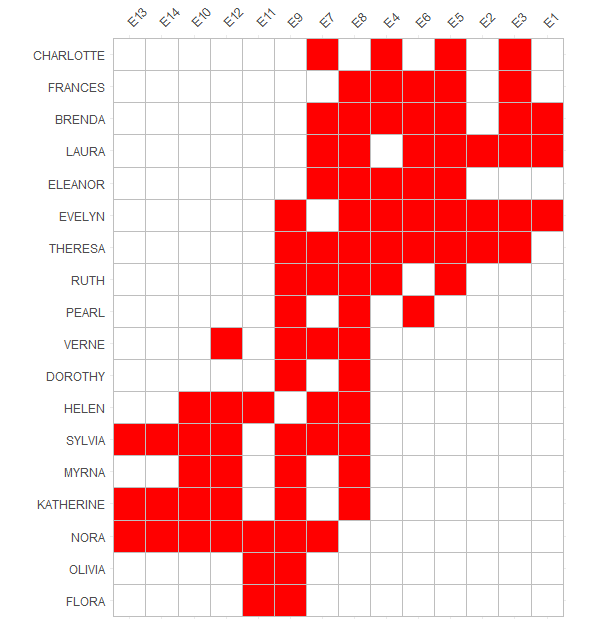
\includegraphics{Plots/sr-plot-reord.png}

}

\caption{SimRank Re-ordered Affiliation Matrix}

\end{figure}
\end{column}

\begin{column}{0.5\textwidth}
\begin{figure}

{\centering 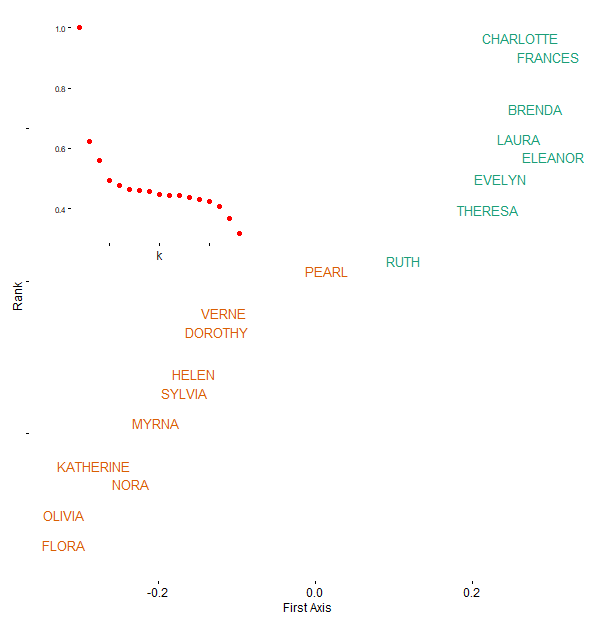
\includegraphics{Plots/sr-plot-eigen-p.png}

}

\caption{Simrank Similarity Matrix Eigenvalue Plot (Persons)}

\end{figure}
\end{column}
\end{columns}
\end{frame}

\begin{frame}{CA and SimRank}
\protect\hypertarget{ca-and-simrank-4}{}
\begin{columns}[T]
\begin{column}{0.5\textwidth}
\begin{figure}

{\centering 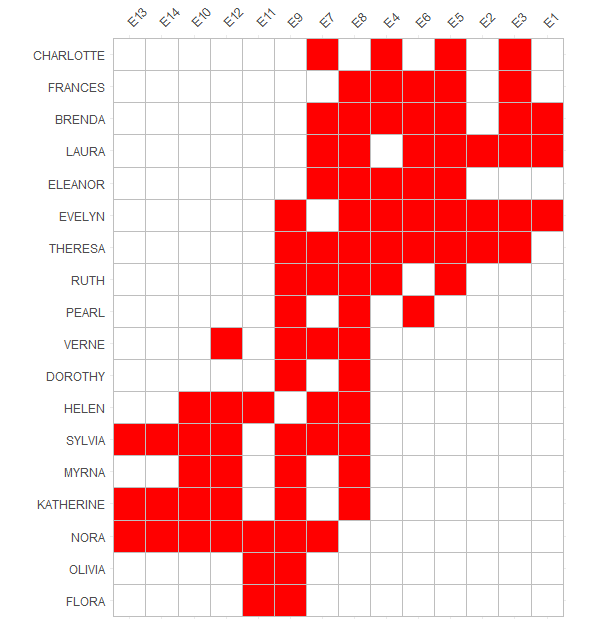
\includegraphics{Plots/sr-plot-reord.png}

}

\caption{SimRank Re-ordered Affiliation Matrix}

\end{figure}
\end{column}

\begin{column}{0.5\textwidth}
\begin{figure}

{\centering 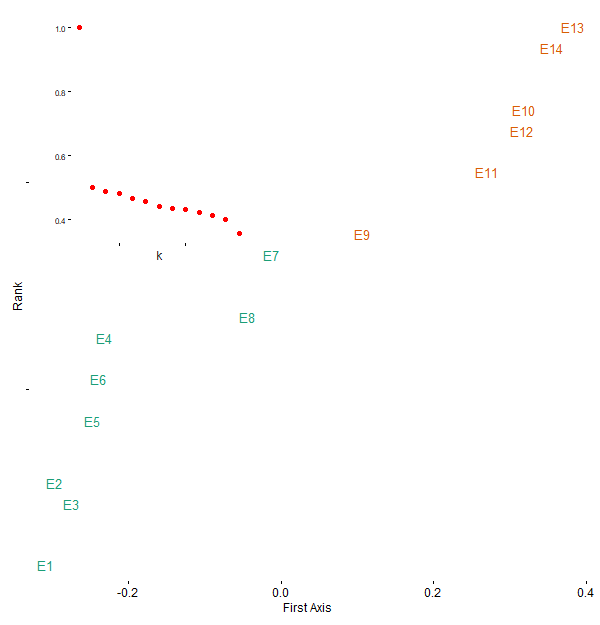
\includegraphics{Plots/sr-plot-eigen-g.png}

}

\caption{Simrank Similarity Matrix Eigenvalue Plot (Groups)}

\end{figure}
\end{column}
\end{columns}
\end{frame}

\begin{frame}{CA and SimRank}
\protect\hypertarget{ca-and-simrank-5}{}
\begin{columns}[T]
\begin{column}{0.5\textwidth}
\begin{figure}

{\centering 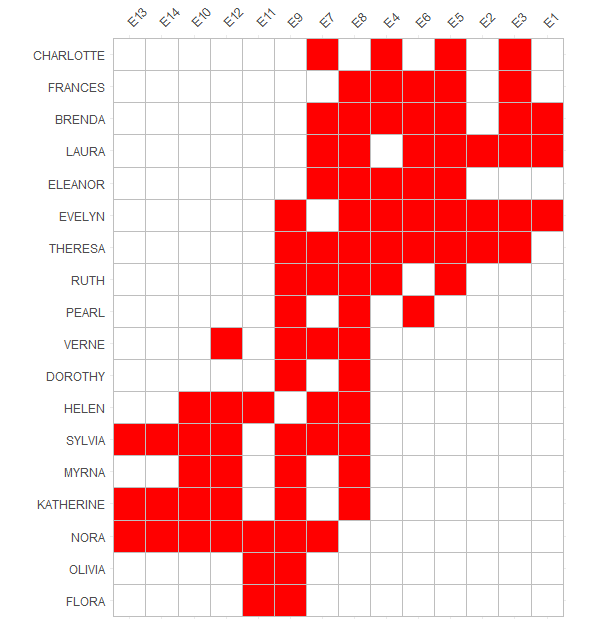
\includegraphics{Plots/sr-plot-reord.png}

}

\caption{SimRank Re-ordered Affiliation Matrix}

\end{figure}
\end{column}

\begin{column}{0.3\textwidth}
\begin{figure}

{\centering 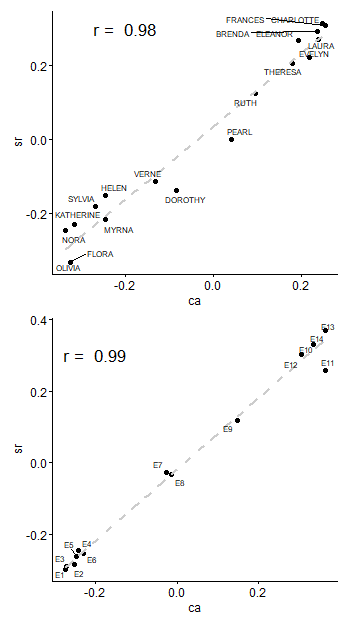
\includegraphics{Plots/sr-corr-scatter.png}

}

\caption{Correlation between CA and SimRank Similarity Matrix
Eigenvectors}

\end{figure}
\end{column}
\end{columns}
\end{frame}

\begin{frame}{CA and Generalized Relational Similarity}
\protect\hypertarget{ca-and-generalized-relational-similarity-1}{}
\begin{itemize}
\item
  I recently proposed a measure of generalized relational similarity
  (GSR) metric for nodes in two-mode networks by ``tweaking'' a previous
  approach based on the modified correlation distance*
\item
  For pairs of people the GSR is given by:
\end{itemize}

\begin{equation}\protect\hypertarget{eq-kovacs1}{}{
\begin{equation}
\scriptsize
    S(p, p') = 
    \frac{
    (A_{p\bullet} - \bar{A}_{p\bullet})
    \mathbf{S(G)}
    (A_{p'\bullet} - \bar{A}_{p'\bullet})^T
    }
    {
    \sqrt{
    (A_{p\bullet} - \bar{A}_{p\bullet})
    \mathbf{S(G)}
    (A_{p\bullet} - \bar{A}_{p\bullet})^T
    }
    \sqrt{
    (A_{p'\bullet} - \bar{A}_{p'\bullet})
    \mathbf{S(G)}
    (A_{p'\bullet} - \bar{A}_{p'\bullet})^T
        }
    }
\end{equation}
}\label{eq-kovacs1}\end{equation}

\begin{itemize}
\tightlist
\item
  And for groups:
\end{itemize}

\begin{equation}\protect\hypertarget{eq-kovacs2}{}{
\begin{equation}
\scriptsize 
    S(g, g') = 
    \frac{
    (A_{g\bullet} - \bar{A}_{g\bullet})
    \mathbf{S(P)}
    (A_{g'\bullet} - \bar{A}_{g'\bullet})^T
    }
    {
    \sqrt{
    (A_{g\bullet} - \bar{A}_{g\bullet})
    \mathbf{S(P)}
    (A_{g\bullet} - \bar{A}_{g\bullet})^T
    }
    \sqrt{
    (A_{g'\bullet} - \bar{A}_{g'\bullet})
    \mathbf{S(P)}
    (A_{g'\bullet} - \bar{A}_{g'\bullet})^T
        }
    }
\end{equation}
}\label{eq-kovacs2}\end{equation}

\marginnote{\begin{footnotesize}

*Lizardo 2024; Kovacs 2010

\end{footnotesize}}
\end{frame}

\begin{frame}{CA and Generalized Relational Similarity}
\protect\hypertarget{ca-and-generalized-relational-similarity-2}{}
\begin{itemize}
\tightlist
\item
  With the base similarities between people given by:
\end{itemize}

\begin{equation}\protect\hypertarget{eq-lizardo1}{}{
\mathbf{S(P)}_{pp'} = \frac{AA_{pp'}}{\sqrt{AA_{pp}AA_{p'p'}}}
}\label{eq-lizardo1}\end{equation}

\begin{itemize}
\tightlist
\item
  And the base similarities for groups:
\end{itemize}

\begin{equation}\protect\hypertarget{eq-lizardo2}{}{
\mathbf{S(G)}_{gg'} = \frac{AA_{gg'}}{\sqrt{AA_{gg}AA_{g'g'}}}
}\label{eq-lizardo2}\end{equation}

\begin{itemize}
\tightlist
\item
  Namely, the cosine distances between people and groups based on the
  corresponding cell entries of the one-mode projections*
\end{itemize}

\marginnote{\begin{footnotesize}

*Lizardo 2024

\end{footnotesize}}
\end{frame}

\begin{frame}{CA and Generalized Relational Similarity}
\protect\hypertarget{ca-and-generalized-relational-similarity-3}{}
\begin{columns}[T]
\begin{column}{0.5\textwidth}
\begin{figure}

{\centering 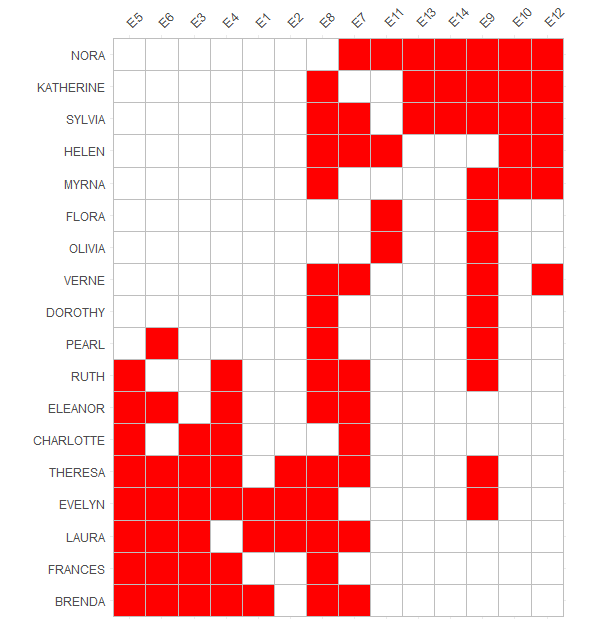
\includegraphics{Plots/grs-plot-reord.png}

}

\caption{GRS Re-ordered Affiliation Matrix}

\end{figure}
\end{column}

\begin{column}{0.5\textwidth}
\begin{figure}

{\centering 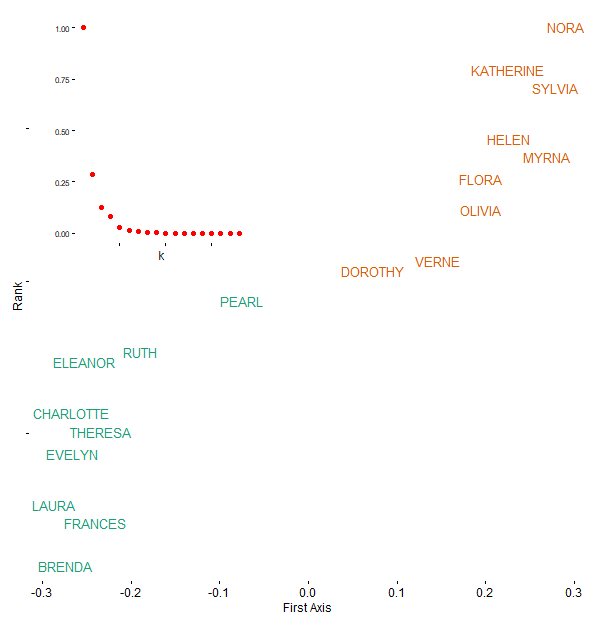
\includegraphics{Plots/grs-plot-eigen-p.png}

}

\caption{GRS Similarity Matrix Eigenvalue Plot (Persons)}

\end{figure}
\end{column}
\end{columns}
\end{frame}

\begin{frame}{CA and Generalized Relational Similarity}
\protect\hypertarget{ca-and-generalized-relational-similarity-4}{}
\begin{columns}[T]
\begin{column}{0.5\textwidth}
\begin{figure}

{\centering 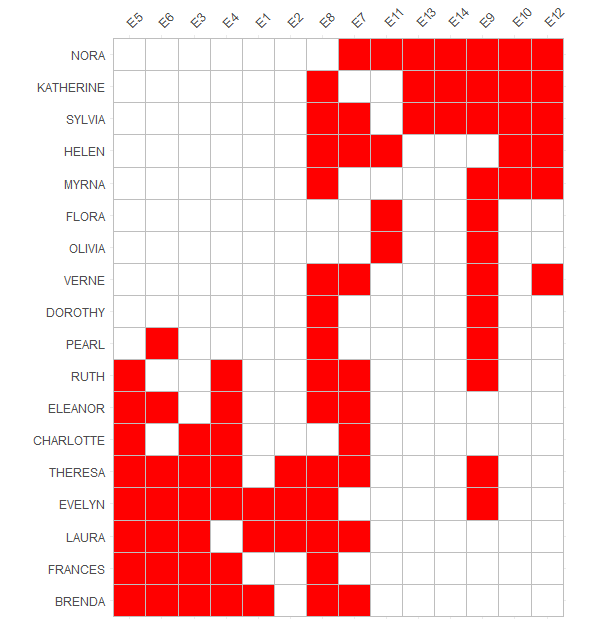
\includegraphics{Plots/grs-plot-reord.png}

}

\caption{GRS Re-ordered Affiliation Matrix}

\end{figure}
\end{column}

\begin{column}{0.5\textwidth}
\begin{figure}

{\centering 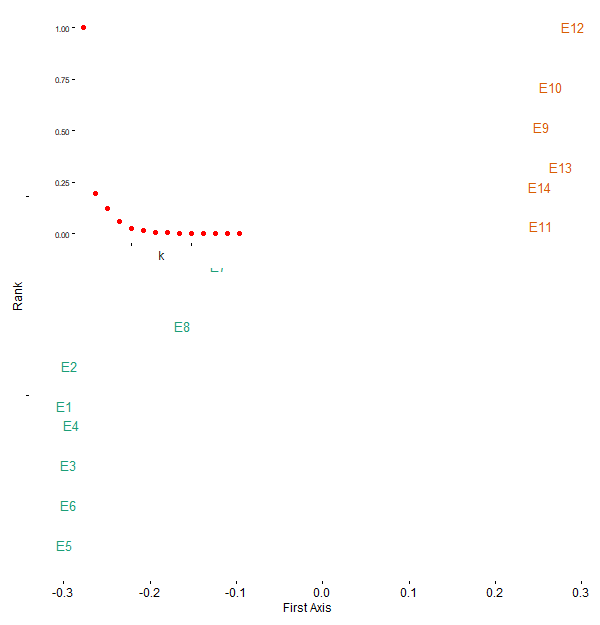
\includegraphics{Plots/grs-plot-eigen-g.png}

}

\caption{GRS Similarity Matrix Eigenvalue Plot (Groups)}

\end{figure}
\end{column}
\end{columns}
\end{frame}

\begin{frame}{CA and Generalized Relational Similarity}
\protect\hypertarget{ca-and-generalized-relational-similarity-5}{}
\begin{columns}[T]
\begin{column}{0.5\textwidth}
\begin{figure}

{\centering 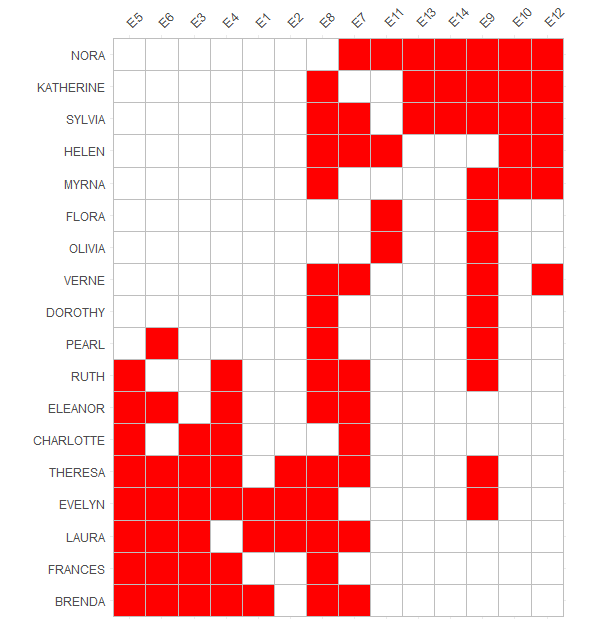
\includegraphics{Plots/grs-plot-reord.png}

}

\caption{GRS Re-ordered Affiliation Matrix}

\end{figure}
\end{column}

\begin{column}{0.3\textwidth}
\begin{figure}

{\centering 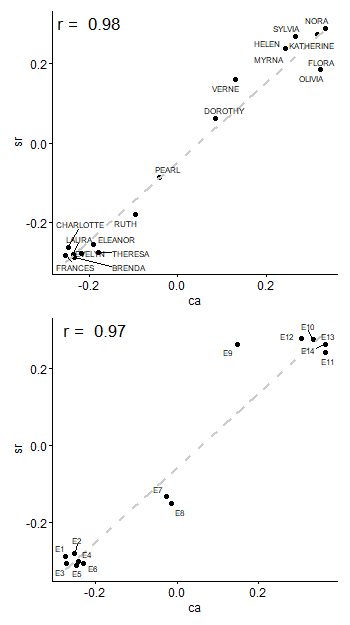
\includegraphics{Plots/grs-corr-scatter.png}

}

\caption{Correlation between CA and GRS Matrix Eigenvectors}

\end{figure}
\end{column}
\end{columns}
\end{frame}

\begin{frame}{Conclusions}
\protect\hypertarget{conclusions}{}
\begin{itemize}
\tightlist
\item
  To paraphrase John Martin paraphrasing Levi-Strauss:

  \begin{itemize}
  \tightlist
  \item
    There is only \emph{one analysis} in two-mode network analysis and
    it is CA
  \item
    Rediscovered many times by researchers pursuing seemingly
    incompatible taks
  \end{itemize}
\end{itemize}

\pause

\begin{itemize}
\tightlist
\item
  Contra skeptics we can do two-mode ``sna'' when we do CA

  \begin{itemize}
  \tightlist
  \item
    Rank nodes against a meaningful centrality metric
  \item
    Detect equivalences (generalized similarities) between node clusters
  \end{itemize}
\item
  These are some of the standard ``positional'' tasks that take up much
  sna
\end{itemize}
\end{frame}

\begin{frame}{Conclusions}
\protect\hypertarget{conclusions-1}{}
\begin{itemize}
\tightlist
\item
  To paraphrase John Martin paraphrasing Levi-Strauss:

  \begin{itemize}
  \tightlist
  \item
    There is only \emph{one analysis} in two-mode network analysis and
    it is CA
  \item
    Rediscovered many times by researchers pursuing seemingly
    incompatible taks
  \end{itemize}
\end{itemize}

\pause

\begin{itemize}
\tightlist
\item
  We can also go do more than visualization and joint display
\item
  The first CA dimension particularly represents a seldom noted
  \textbf{duality of ranking and equivalence}

  \begin{itemize}
  \tightlist
  \item
    Ranking via similarity within clusters
  \item
    Bonacich by contrast is a ``pure'' centrality ranking
  \end{itemize}
\end{itemize}
\end{frame}

\begin{frame}{Conclusions}
\protect\hypertarget{conclusions-2}{}
\begin{itemize}
\tightlist
\item
  To paraphrase John Martin paraphrasing Levi-Strauss:

  \begin{itemize}
  \tightlist
  \item
    There is only \emph{one analysis} in two-mode network analysis and
    it is CA
  \item
    Rediscovered many times by researchers pursuing seemingly
    incompatible taks
  \end{itemize}
\end{itemize}

\pause

\begin{itemize}
\tightlist
\item
  Using CA for this kind of ``spectral clustering'' and ``spectral
  ranking'' is not common but feasible

  \begin{itemize}
  \tightlist
  \item
    Another approach (similar to blockmodeling):

    \begin{itemize}
    \tightlist
    \item
      Use CA for spectral clustering
    \item
      Then use \textbf{specific CA} (on sub-tables defined by the
      eigengap heuristic) to split clusters into further clusters
    \end{itemize}
  \end{itemize}
\end{itemize}
\end{frame}

\begin{frame}{Thanks!}
\protect\hypertarget{thanks}{}
\url{https://github.com/olizardo/correspondence-analysis-two-mode-networks}

olizardo@soc.ucla.edu
\end{frame}



\end{document}
